\documentclass[unnumsec,webpdf,contemporary,large]{oup-authoring-template}
%% OUP authoring template (v1.5), bundled so that this package compiles
%% directly on Overleaf without installing extra class files.
%% Highlighted revision version (BIB-26-2683 Major Revision): all revised or
%% newly added passages are marked in blue via \rev{...}.

\usepackage[T1]{fontenc}
\usepackage{lmodern}
\usepackage{booktabs}
\usepackage{graphicx}
\usepackage{amsmath}
\usepackage{amssymb}
\usepackage{textcomp}
\PassOptionsToPackage{hyphens}{url}
\usepackage{url}
\usepackage{microtype}
\usepackage{placeins}
\usepackage{xcolor}
\usepackage[hidelinks]{hyperref}

%% Toggle highlight color for Marked vs Clean manuscript PDFs:
\newcommand{\rev}[1]{\textcolor{blue}{#1}}
\pdfstringdefDisableCommands{\def\rev#1{#1}}
\setlength{\emergencystretch}{1.5em}

\def\societylogo{}

\usepackage{etoolbox}
\makeatletter
\patchcmd{\ps@opening}{\vskip2.5pt\hbox to \textwidth}{\vskip2.5pt\hbox to \dimexpr\textwidth-4mm\relax}{}{\PackageError{bib-revision}{Opening odd header patch failed}{Inspect the bundled class.}}
\patchcmd{\ps@opening}{\vskip2.5pt\hbox to \textwidth}{\vskip2.5pt\hbox to \dimexpr\textwidth-4mm\relax}{}{\PackageError{bib-revision}{Opening even header patch failed}{Inspect the bundled class.}}
\def\ps@opening{\def\@oddhead{\small\itshape Briefings in Bioinformatics\hfill Problem solving protocol}\let\@evenhead\@oddhead\def\@oddfoot{\hfil\thepage\hfil}\let\@evenfoot\@oddfoot}
\def\ps@manuscript{\def\@oddhead{\small\itshape Reconstruction and generation in AMP design\hfill\thepage}\let\@evenhead\@oddhead\let\@oddfoot\@empty\let\@evenfoot\@empty}
\makeatother

\graphicspath{{figures/}}

\hypersetup{pdfauthor={Hongsheng Wang, Zihan Zeng, Fei Wu, Feng Lin and Xingxu Huang}}
\begin{document}

\journaltitle{Briefings in Bioinformatics}
\DOI{}
\copyrightyear{2026}
\pubyear{2026}
\vol{}
\issue{}
\access{}
\appnotes{Problem solving protocol}
\firstpage{1}

\title[Reconstruction and generation in AMP design]{Separating reconstruction, generation and antibacterial activity in antimicrobial peptide design}

\author[1,2,$\ast$]{Hongsheng Wang\ORCID{0009-0009-8214-5150}}
\author[3]{Zihan Zeng}
\author[1]{Fei Wu\ORCID{0000-0003-2139-8807}}
\author[4]{Feng Lin\ORCID{0000-0002-1199-5870}}
\author[5]{Xingxu Huang\ORCID{0000-0001-8934-1247}}

\address[1]{\orgdiv{College of Computer Science and Technology}, \orgname{Zhejiang University}, \orgaddress{\street{866 Yuhangtang Road, Xihu District}, \postcode{310058}, \state{Zhejiang}, \country{China}}}
\address[2]{\orgdiv{Artificial Intelligence Department}, \orgname{Loctek Ergonomic Technology Corp.}, \orgaddress{\street{Loctek Building, 436 Xueshi Road, Shounan Subdistrict, Yinzhou District}, \postcode{315100}, \state{Zhejiang}, \country{China}}}
\address[3]{\orgdiv{Polytechnic Institute}, \orgname{Zhejiang University}, \orgaddress{Hangzhou, \postcode{310015}, \country{China}}}
\address[4]{\orgname{Fuyao University of Science and Technology}, \orgaddress{\street{No. 104 Zhihui Avenue, Fuzhou High-tech Industrial Development Zone}, \postcode{350109}, \state{Fujian}, \country{China}}}
\address[5]{\orgdiv{Laboratory of Pancreatic Disease}, \orgname{The First Affiliated Hospital, Zhejiang University School of Medicine}, \orgaddress{Hangzhou, \postcode{310058}, \country{China}}}
\corresp[$\ast$]{Correspondence: Hongsheng Wang. \href{mailto:wanghongsheng@zju.edu.cn}{wanghongsheng@zju.edu.cn}}

\abstract{Antimicrobial peptide (AMP) design combines sequence reconstruction, de novo generation and experimental activity assessment, yet each endpoint answers a distinct evaluation question. We present an endpoint-specific evaluation protocol \rev{validated across both our original homology-partitioned pilot cohort (279 training and 41 development peptides) and an 11-fold larger, strictly homology-isolated DBAASP benchmark (3,565 peptides; 3,120 training, 223 validation and 222 untouched independent test peptides with zero cross-split identity $\geq$70\%). Across multi-seed experiments (3--5 seeds, 128--256 samples per terminal condition) spanning statistical baselines (unigram, bigram and trigram Markov models), capacity-matched autoregressive generators (LSTM-small, LSTM-matched and Transformer-LM), non-diffusion GRU-VAEs and matched VAE--diffusion models, we show that hyperparameter tuning (KL weight $\beta=0.1$, 21-fold MSE scaling and higher learning rate) elevates independent-test reconstruction accuracy to 96.05$\pm$0.64\% for categorical cross-entropy (CE21) and 94.24$\pm$0.69\% for tuned squared-error (MSE21). Nevertheless, de novo sampling from both tuned VAE--diffusion pipelines still trails capacity-matched autoregressive generators by roughly 20-fold on free-terminus MMD$^2$ (0.0654--0.0671 versus 0.0032--0.0036). Correlation auditing reveals that six low-order distances span only 1.54 effective dimensions (PC1+PC2 = 95.3\%), whereas tripeptide divergence, $\alpha$-helical hydrophobic moment ($\mu_H$) and $\geq$70\% nearest-neighbor alignment identity separate neural generators from unigram sampling ($p\leq 0.028$) and expose hidden near-duplicate collapse (up to 34.1\% despite 0\% exact copies).} In a separate, provenance-documented panel of 27 peptides assayed by Mueller--Hinton broth microdilution, six inhibit \textit{Staphylococcus aureus} ATCC 29213 at MICs $\leq$31.25 \textmu{}g/mL \rev{(3.09--12.87 \textmu{}M), a count invariant across five OD$_{600}$ and blank-normalized growth thresholds; haemolysis and cytotoxicity remain unmeasured.} Separating reconstruction, multi-dimensional sampling and wet-lab endpoints yields a practical, reproducible standard for AMP design studies.}

\keywords{antimicrobial peptides, generative models, evaluation, variational autoencoder, diffusion models, antibacterial activity}

\otherabstract[Author description]{The authors study machine learning for antimicrobial peptide discovery across computer science, industrial artificial intelligence and biotechnology, emphasizing reproducible evaluation of computational design and laboratory measurements.}

\maketitle
\pagestyle{manuscript}
\raggedbottom

\section{Introduction}

Antimicrobial peptides (AMPs) provide diverse sequence templates for antibacterial discovery, with activity shaped by sequence, structure and experimental context \cite{ref50,ref51}. Recurrent models \cite{ref1}, variational autoencoders \cite{ref16,ref17,ref2}, conditional adversarial models \cite{ref15,ref19} and diffusion approaches \cite{ref9,ref11,ref20} explore this sequence space through distinct generative mechanisms, while integrated frameworks combine generation, identification, activity prediction and optimization \cite{ref21}. \rev{Complementing generative architectures, representation-learning and sequence-based feature-optimization studies across peptides and proteins demonstrate how deeply learned embeddings and engineered physicochemical descriptors capture distinct aspects of primary-sequence organization \cite{refLe2022,refLe2021,refAMPScanner}.}

Computational design becomes biologically informative when generated or screened sequences are connected to explicit functional measurements. Workflows combining generative models with molecular simulations \cite{ref14,refCao2023}, large-scale sequence screening \cite{ref22} and staged selection followed by broth microdilution assays, as in AMPGen \cite{ref9}, contain distinct generation, candidate-selection and experimental-validation stages \cite{ref25}. A recurring methodological hazard is treating an improvement at one stage as evidence for another: sequence reconstruction measures recovery of a known peptide from an encoded representation; de novo generation samples without access to target sequences or residue-aligned descriptors; and minimum inhibitory concentration (MIC) assays test whether a specific filtered candidate inhibits a specified strain under defined laboratory conditions.

\rev{While this conceptual distinction is recognized in principle, existing benchmarking frameworks leave an operational gap for AMP design (\textbf{Table 1}). Small-molecule benchmarks such as MOSES \cite{ref26} and GuacaMol \cite{ref28} standardize low-order distributional statistics without peptide-specific homology leakage control or wet-lab MIC auditing. Recent biological sequence evaluation libraries such as \texttt{seqme} \cite{ref29} and comparative AMP surveys \cite{ref8} evaluate sampling quality across model families, whereas QMAP \cite{ref13} benchmarks supervised MIC and haemolytic regression and DOME \cite{ref43} provides general supervised-ML checklists \cite{ref44,ref45}. AMP classification audits further show how model complexity, negative-data selection and sequence homology bias apparent performance \cite{refXu2021,ref4,ref5,ref39,ref40}, while species-aware language models highlight strain specificity \cite{refLLAMP}. However, no single protocol operationally integrates (i) hyperparameter- and padding-controlled reconstruction attribution, (ii) multi-seed de novo sampling audited against simple statistical baselines, capacity-matched architectures, metric-redundancy dimensionality, $\alpha$-helical amphipathicity and near-homolog memorization on homology-isolated test sets, and (iii) provenance-explicit wet-lab MIC reporting with multi-threshold OD$_{600}$ sensitivity checks.}

\begin{table*}[t]
\caption{\rev{Comparison of the proposed endpoint-specific evaluation protocol with existing benchmarking frameworks and explicit scope/overlap accounting relative to our previously published AMPGen study \cite{ref9}.}}
\label{tab:framework_overlap}
\centering
\footnotesize
\begin{tabular}{>{\raggedright\arraybackslash}p{2.7cm}>{\raggedright\arraybackslash}p{3.0cm}>{\raggedright\arraybackslash}p{3.0cm}>{\raggedright\arraybackslash}p{3.1cm}>{\raggedright\arraybackslash}p{3.3cm}}
\toprule
\rev{Framework / Study} & \rev{Primary Scope} & \rev{Homology / Leakage Control} & \rev{Generation \& Memorization Gates} & \rev{Relation / Overlap with Present Work} \\
\midrule
\rev{MOSES \cite{ref26}; GuacaMol \cite{ref28}} & \rev{Small-molecule SMILES generation} & \rev{Random split; exact copy check} & \rev{Low-order distributional metrics; novelty} & \rev{Conceptual origin of multi-metric generation benchmarks; no peptide endpoints} \\
\rev{\texttt{seqme} \cite{ref29}; Beierle et al. \cite{ref8}} & \rev{Biological sequence / AMP generation} & \rev{Benchmark-dependent} & \rev{Composition, length, classifier scores} & \rev{Complementary sampling metrics; does not pair controlled reconstruction ablations or MIC OD$_{600}$ audits} \\
\rev{QMAP \cite{ref13}; DOME \cite{ref43}} & \rev{Supervised MIC regression / ML checklists} & \rev{Homology / source grouping} & \rev{Not applicable (predictive only)} & \rev{Informs our source-group activity regression and reporting transparency} \\
\rev{AMPGen (Jin et al., 2025) \cite{ref9}} & \rev{Evolutionary + diffusion AMP generator; 38-peptide staged MIC + toxicity assays} & \rev{6-database pool (10,249 AMPs); DBAASP MIC subset (3,929 items)} & \rev{Sequence/property screening; staged 2-strain $\rightarrow$ 4-strain wet-lab} & \rev{Shared co-authors (4/5); \textbf{distinct architecture}, \textbf{separate datasets}, \textbf{0/27 candidate sequence overlap}, \textbf{separate assays} sharing identical MHB microdilution protocol} \\
\rev{\textbf{Present Protocol}} & \rev{Unified 3-endpoint protocol (reconstruction, generation, MIC audit)} & \rev{$\leq$70\% global NW transitive clustering; strict untouched test set} & \rev{Multi-seed CI, statistical baselines, capacity-matched AR, $d_{\mathrm{eff}}$, 3-mer, $\mu_H$, $\geq$70\% NW memorization} & \rev{Separates Primary, Exploratory and Retrospective tiers with hash-bound reproducibility} \\
\bottomrule
\end{tabular}
\end{table*}

\rev{In this Problem Solving Protocol, we address these gaps through a two-scale, multi-seed evaluation study. First, retaining our original 279-training/41-development pilot cohort for continuity, we construct an 11-fold larger, frozen DBAASP benchmark (3,565 peptides; 3,120 training, 223 validation and 222 untouched independent test peptides with zero cross-split identity $\geq$70\%). Second, we test whether categorical cross-entropy (CE21) gains over squared-error (MSE21) reconstruction persist under tuned KL regularization ($\beta\in\{0.01,0.1,1.0\}$), 21-fold MSE loss rescaling, higher learning rates and padding masking, and evaluate whether near-perfect reconstruction translates into de novo generation quality against statistical baselines (unigram, bigram and trigram Markov), capacity-matched autoregressive generators (LSTM-matched and Transformer-LM) and non-diffusion GRU-VAEs. Third, we audit metric redundancy, higher-order sequence organization, amphipathicity and near-duplicate memorization, and pair these computational endpoints with a fully documented, provenance-explicit 27-peptide broth microdilution case study.}

\section{Materials and methods}

\rev{\subsection{Study organization: primary, exploratory and retrospective tiers}}

\rev{To prevent conflating confirmatory comparisons with diagnostic probes, every analysis is assigned to one of three explicit tiers: \textbf{(i) Primary analyses}, comprising multi-seed reconstruction and de novo generation on the strictly untouched expanded DBAASP independent test set ($n=222$), multi-seed hyperparameter/padding ablations, large-sample replay of the original pilot checkpoints ($256\times 5$ samples per terminal), and the primary original MIC summary of the 27-peptide panel; \textbf{(ii) Exploratory diagnostic analyses}, comprising the seven latent-space perturbation routes (Table S4) and source-group activity-regression screens (Table S3), included specifically to diagnose mechanisms underlying the Endpoint 1--2 gap and why in-silico predictors cannot substitute for Endpoint 3; and \textbf{(iii) Retrospective sensitivity analyses}, comprising the multi-threshold OD$_{600}$ and blank-normalized growth-inhibition audit of the 3,240 laboratory optical-density readings.}

\subsection{Peptide datasets, homology partitioning and terminal conditions}

\textbf{Original pilot cohort (279 training / 41 development).} We retained the original 320-peptide computational cohort derived from 512 DBAASP detail cards \cite{ref10} to ensure exact continuity with our initial submission. Eligibility required an unmodified canonical L-amino-acid monomer of 1--48 residues, an unmodified N terminus, a free (FREE) or amidated (AMD) C terminus, valid RDKit molecular graphs and bacterial MIC metadata. Sequences were clustered by global Needleman--Wunsch alignment \cite{refNW} (match $+2$, mismatch $-1$, gap $-2$; identity = matches / all alignment columns including gaps) at $\geq$70\% identity into transitive connected components, yielding 279 training sequences (126 FREE, 153 AMD) and 41 development sequences (18 FREE, 23 AMD; 701 non-padding residues). Because the 41-peptide development split was consulted during model development, all pilot comparisons are explicitly designated descriptive.

\rev{\textbf{Expanded homology-isolated DBAASP benchmark (3,120 training / 223 validation / 222 independent test).} To establish generalizability across an order-of-magnitude larger cohort with a strictly untouched independent test set, we retrieved 4,399 unique monomer antibacterial peptide records (Gram-positive and Gram-negative targets) from the official DBAASP REST API (\url{https://dbaasp.org/peptides}, frozen snapshot 25 November 2026, SHA-256 archived in Table S7). Applying the identical eligibility filters removed 602 non-canonical sequences, 128 N-terminally modified peptides, 81 sequences exceeding 48 residues and 3 non-FREE/AMD C-terminal variants, yielding 3,565 unique eligible (sequence, terminal-state) records (3,492 unique sequences; zero RDKit graph failures). Exact $\geq$70\% global Needleman--Wunsch transitive clustering partitioned these 3,492 sequences into 1,106 connected components. All 59 components sharing an exact sequence with the pilot cohort and all 56 records with $\geq$70\% identity to any pilot sequence were assigned exclusively to training; remaining components were partitioned by deterministic SHA-256 hash into \textbf{3,120 training} (1,727 FREE, 1,393 AMD; 61,166 residues; 883 components), \textbf{223 validation} (146 FREE, 77 AMD; 4,497 residues; 116 components) and \textbf{222 untouched independent test} sequences (135 FREE, 87 AMD; 5,083 residues; 107 components; 0 sequences $<$5 aa). Exhaustive pairwise verification confirmed \textbf{zero} sequence pairs with $\geq$70\% global identity between the independent test set and any training, validation or pilot sequence. Descriptor standardization (RDKit per-residue MolWt, MolLogP, TPSA and nine full-peptide global descriptors) used training data only. Terminal state (FREE vs AMD) was the sole external conditioning input during de novo generation.}

\subsection{Models, hyperparameter ablations and capacity-matched comparators}

\textbf{Matched VAE--diffusion pipelines and objective ablations.} The categorical (CE21) and squared-error (MSE21) pipelines used the identical flow-guided convolutional VAE \cite{refVAE} (1,681,549 parameters; 48-position output, 21-category head for 20 canonical amino acids plus padding, legal-prefix decoding) paired with a 2D U-Net conditional latent denoiser \cite{refDDPM} (18,612,994 parameters) trained on stacked posterior parameters $(\mu, \log\sigma)$. Let $s_{ijc}$ denote the raw score for class $c$ at position $j$ of sample $i$, $y_{ij}$ the target class and $B$ the batch size:
\begin{align*}
\mathcal{L}_{\mathrm{CE}} &= -\frac{1}{48B}\sum_{i}\sum_{j}\log \operatorname{softmax}(s_{ij})_{y_{ij}}, \\
\mathcal{L}_{\mathrm{MSE}} &= \frac{\alpha}{48B}\sum_{i}\sum_{j}\bigl\lVert s_{ij} - e_{y_{ij}} \bigr\rVert^{2},
\end{align*}
where $e_y$ is the one-hot target and $\alpha=0.5$ is the default prefactor. \rev{Because raw MSE21 differs from CE21 in per-position gradient magnitude and effective KL regularization, we conducted a systematic 3-seed hyperparameter sweep across KL weights $\beta\in\{0.01, 0.1, 1.0\}$ for both CE21 and MSE21, plus a \textbf{tuned MSE21} configuration ($\alpha=10.5$, representing 21-fold loss rescaling to equalize per-position scale with CE21, paired with a 4-fold higher learning rate of $2\times 10^{-3}$). To isolate the influence of padding on reconstruction (approximately 64\% of positions in the 48-residue grid are padding), we ran 3-seed padding-masked ablations excluding padding positions from $\mathcal{L}_{\mathrm{CE}}$ and $\mathcal{L}_{\mathrm{MSE}}$ and evaluated both legal-prefix decoding and oracle-length non-padding accuracy. On the expanded DBAASP benchmark, we trained 3-seed full VAE--DDPM pipelines (seeds 222, 333, 444; 300 VAE + 300 DDPM updates; 128 generated sequences per terminal condition via 15-step DDIM sampling) for default CE21 ($\beta=1.0$), tuned CE21 ($\beta=0.1$), default MSE21 ($\beta=1.0$) and tuned MSE21 ($\beta=0.1$, $\alpha=10.5$, LR $2\times 10^{-3}$).}

\rev{\textbf{Statistical baselines, capacity-matched autoregressive models and non-diffusion VAEs.} To control for model capacity, inductive bias and low-data suitability, we evaluated eight additional comparators across 5 independent random seeds (222, 333, 444, 555, 666) with \textbf{256 generated sequences per terminal condition} (2,560 generated peptides per model per cohort) on both the pilot and expanded benchmarks:
\begin{enumerate}
\item \textit{Three closed-form statistical baselines} (0 learned neural parameters): terminal-conditioned empirical length + 0-order amino-acid sampling (\textbf{Unigram}), 1st-order Markov language model with Laplace smoothing $\alpha=0.5$ (\textbf{Bigram Markov}) and 2nd-order Markov model with bigram backoff (\textbf{Trigram Markov}).
\item \textit{Three autoregressive neural architectures} (validation-checkpointed on the expanded benchmark): the original 2-layer \textbf{LSTM-small} (hidden width 64; 62,501 parameters \cite{refLSTM}), a capacity-matched 2-layer \textbf{LSTM-matched} (hidden width 320, dropout 0.15; 1,344,501 parameters) and a capacity-matched 4-layer causal \textbf{Transformer-LM} ($d_{\mathrm{model}}=192$, 4 attention heads, FFN width 768, dropout 0.15; 1,797,717 parameters).
\item \textit{Two matched non-diffusion sequence VAEs} (2-layer bidirectional GRU encoder + 2-layer GRU decoder, latent width 64, $\beta=0.1$; 1,992,549 parameters) trained with CE21 (\textbf{GRU-VAE CE21}) versus MSE21 (\textbf{GRU-VAE MSE21}), testing whether reconstruction-versus-generation separation generalizes to a standard recurrent VAE architecture without latent diffusion.
\end{enumerate}
Finally, to test sample-size stability of our exact original v7 checkpoints without retraining, we reloaded all four frozen v7 models (CE21\_DDPM, MSE21\_DDPM, scalar\_DDPM and terminal\_LSTM) and generated $256\times 5$ sequences per terminal condition (1,280 per terminal; 80-fold more sequences than the original 16).}

\subsection{Orthogonal evaluation metrics and uncertainty estimation}

Reconstruction was evaluated from the posterior mean using non-padding residue micro accuracy, unweighted amino-acid macro recall across supported classes, length MAE and whole-sequence exact match. \rev{For de novo generation, we retained the six original low-order distances (residue and dipeptide Jensen--Shannon divergence \cite{refJS} in bits, residue and dipeptide $L_1$ distances, length Kolmogorov--Smirnov statistic and biased linear-kernel MMD$^2$ \cite{refMMD}) and audited their mutual redundancy across 160 model--seed--terminal evaluations via Spearman rank correlation and principal component analysis (PCA) participation-ratio effective dimensionality $d_{\mathrm{eff}} = (\sum \lambda_k)^2 / \sum \lambda_k^2$. To capture higher-order organization, biological relevance and memorization beyond exact string matches, we added: (i) \textbf{tripeptide (3-mer) JS divergence} (bits); (ii) \textbf{Wasserstein-1 distances} between generated and reference distributions for AMP-relevant physicochemical and structural properties---net charge at pH 7.4 (explicitly modeling FREE vs AMD C-termini), Eisenberg hydrophobicity, $\alpha$-helical hydrophobic moment $\mu_H$ (100$^\circ$ per residue) \cite{refEisenberg}, Boman protein-binding potential \cite{refBoman}, aliphatic index and aromaticity; (iii) \textbf{nearest-neighbor global Needleman--Wunsch identity} to the training set (mean, 95th percentile, fraction $\geq$70\% near-homologs and exact-copy fraction); (iv) \textbf{internal pairwise diversity} ($1 - \text{mean pairwise global identity}$); and (v) \textbf{short-sequence filtering sensitivity}, recomputing distances after excluding biologically implausible fragments of length 1--4 residues. Multi-seed metrics are reported as mean $\pm$ SD with $t$-based 95\% confidence intervals; pairwise model contrasts use two-sided paired $t$-tests and exact sign-flip permutation tests across matched seeds.}

\subsection{Antibacterial activity assays: provenance, confirmed protocol and sensitivity audit}

\rev{\textbf{Candidate provenance and 1,000$\rightarrow$30$\rightarrow$27 selection funnel.} The 27 experimentally assayed peptides form an independent historical validation panel generated by our earlier multimodal flow-guided VAE--diffusion pipeline (commit \texttt{e7486fb}) trained across three target-spectrum groups (Group 1: broad-spectrum; Group 2: Gram-positive-specific; Group 3: Gram-negative-specific); they are \emph{not} a head-to-head wet-lab assay of CE21, MSE21 and LSTM outputs. From 1,000 initially sampled candidates, sequential in-silico filtering retained sequences with positive RDKit net charge at pH 7.4, AMP Scanner v2 probability $>0.9$ \cite{refAMPScanner}, Guruprasad instability index between 10 and 40, and $\leq$70\% sequence similarity to the training set. After removing exact duplicates and replacing two sequences flagged for synthesis difficulty, 30 peptides were ordered across the three design groups (8, 8 and 14) and 27 were successfully synthesized by solid-phase peptide synthesis (7, 8 and 12; HPLC purity 95.0--99.1\% for 26 peptides and 80.3\% for pp1-7; Table S5a). Programmatic alignment verified \textbf{0/27 sequence overlap} with AMPGen \cite{ref9} and a maximum global identity of 58.3\% (mean 42.8\%, 0\% $\geq$70\%) against all 3,492 unique sequences in our expanded DBAASP benchmark.}

\rev{\textbf{Confirmed broth microdilution MIC protocol.} MIC testing against \textit{Escherichia coli} ATCC 25922, \textit{Pseudomonas aeruginosa} ATCC 27853, \textit{Staphylococcus aureus} ATCC 29213 and \textit{Enterococcus faecalis} ATCC 29212 followed the identical broth microdilution protocol established in our laboratory for AMPGen \cite{ref9,ref64,ref65,ref66}. Synthesized peptides were dissolved in 1\% DMSO and subjected to ten two-fold serial dilutions across columns 1--10 of sterile 96-well plates in Mueller--Hinton Broth (MHB; final tested concentrations 1000 down to 1.953125 \textmu{}g/mL, 50 \textmu{}L/well), with column 11 serving as bacterial growth control (MHB plus inoculum) and column 12 as sterile medium blank (MHB only). Overnight cultures grown in MHB at 37~$^\circ$C with shaking were diluted to $1.0\times 10^6$ CFU/mL in MHB, and 50 \textmu{}L aliquots were added to columns 1--11 (final inoculum $5.0\times 10^5$ CFU/mL; final well volume 100 \textmu{}L). Plates were incubated at 37~$^\circ$C for 16--20 h, with three replicate wells per peptide, strain and concentration (3,240 peptide OD$_{600}$ readings). Ampicillin, polymyxin B and daptomycin served as positive reference antibiotics. The original MIC was defined as the lowest tested concentration precluding bacterial growth after incubation.}

\rev{\textbf{Multi-threshold OD$_{600}$ sensitivity audit and molar conversion.} Alongside the original reported MIC summary, we audited all 3,240 OD$_{600}$ readings using a replicate-consensus rule ($\geq$2 of 3 replicates agreeing) across six inhibition criteria: fixed OD$_{600} < 0.08, 0.10, 0.12$ and $0.15$, plus blank-corrected normalized growth $(\mathrm{OD}_{600}-\mathrm{blank})/(\mathrm{control}-\mathrm{blank}) < 10\%$ and $<20\%$. Non-numeric cells (N) were retained explicitly without zero-imputation. All primary active MICs are reported in both mass (\textmu{}g/mL) and molar (\textmu{}M) units using theoretical peptide molecular weights; $\leq$31.25 \textmu{}g/mL corresponds to the standard two-fold dilution below 32 \textmu{}g/mL (3.09--12.87 \textmu{}M for the active hits, matching benchmark therapeutic-hit ranges), whereas $<$200 \textmu{}g/mL is retained only as a secondary broad-screen threshold alongside full dilution-ladder counts (Table S5f).}

\rev{\subsection{Consolidated five-step evaluation protocol}}
\rev{Practitioners applying this protocol follow five sequential steps: \textbf{(1) Homology-isolated data partitioning} ($\leq$70\% global NW transitive components with a locked independent test set and train-only feature scaling); \textbf{(2) Controlled Endpoint-1 reconstruction ablations} (matched architecture/decoding across KL-$\beta$, loss-scale and padding-mask settings, reporting both micro accuracy and per-residue macro recall); \textbf{(3) Multi-seed Endpoint-2 generation benchmarking} ($\geq$3--5 seeds, $\geq$128--256 samples per condition, 95\% CIs, simple statistical baselines and capacity-matched neural comparators); \textbf{(4) Orthogonal fidelity and memorization gating} (reporting metric $d_{\mathrm{eff}}$ alongside 3-mer JS, $\alpha$-helical $\mu_H$, charge $W_1$, $\geq$70\% NW nearest-neighbor identity, internal diversity and $<$5 aa filtering); and \textbf{(5) Provenance-explicit Endpoint-3 reporting} (full screening funnel, complete broth-microdilution parameters, tested-panel denominators, molar equivalents, multi-threshold OD$_{600}$ sensitivity and explicit disclosure of unmeasured toxicity endpoints). Executable verification scripts are documented in Supplementary Methods.}

\begin{figure*}[!t]
\centering
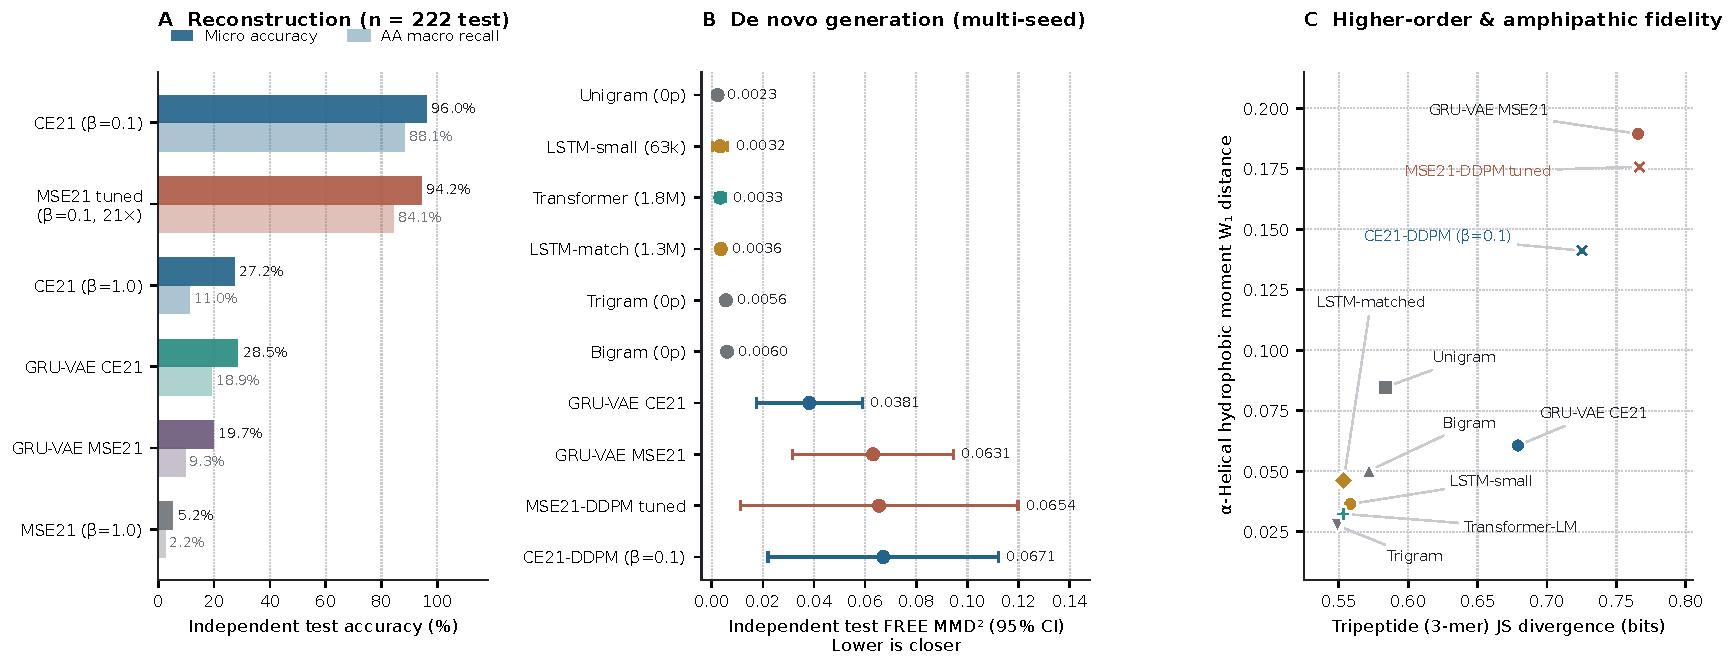
\includegraphics[width=\textwidth]{figures/fig1_multiseed_expanded_benchmark.pdf}
\caption{\rev{Multi-seed reconstruction and de novo generation on the untouched 222-peptide expanded DBAASP independent test set ($<$70\% homology to 3,120 training peptides). \textbf{(A)} Posterior-mean residue micro accuracy (solid) and amino-acid macro recall (faint) across VAE configurations (3--5 seeds). Tuning KL weight ($\beta=0.1$) and 21-fold MSE scaling elevates reconstruction to 96.0\% (CE21) and 94.2\% (MSE21 tuned). \textbf{(B)} De novo FREE-terminus MMD$^2$ (mean and 95\% CI; 128--256 samples per terminal across 3--5 seeds). Both tuned high-reconstruction VAE--DDPM pipelines remain $\sim$20-fold worse than autoregressive models (LSTM-small, LSTM-matched, Transformer-LM). \textbf{(C)} Higher-order tripeptide (3-mer) JS divergence versus $\alpha$-helical hydrophobic moment ($\mu_H$) Wasserstein-1 distance, showing that neural autoregressive models significantly outperform Unigram sampling on sequence organization and amphipathicity ($p\leq 0.028$) despite similar low-order MMD$^2$. Full numerical results appear in Table 3 and Tables S8--S9.}}\par\smallskip{\small\textbf{Alt text:} \rev{Three-panel figure on the 222-peptide independent test set. Panel A shows horizontal bars of reconstruction accuracy reaching 96.0\% for CE21 (beta 0.1) and 94.2\% for tuned MSE21. Panel B shows multi-seed generation MMD squared with 95\% confidence intervals, where LSTM-small, Transformer-LM and LSTM-matched cluster near 0.0032 to 0.0036 versus 0.0654 to 0.0671 for tuned VAE-DDPM. Panel C plots tripeptide JS divergence against alpha-helical hydrophobic moment Wasserstein distance, separating autoregressive models at the lower left from Unigram and VAE-based models.}}
\end{figure*}

\section{Results}

\subsection{Hyperparameter tuning, padding dilution and class imbalance in reconstruction}

\rev{In our original single-seed pilot comparison (1,000 updates, $\beta=1.0$, $\alpha=0.5$), CE21 reconstructed 497/701 development residues (70.90\% micro, 42.76\% macro, length MAE 0.000, 3/41 exact) versus 88/701 (12.55\% micro, 3.57\% macro, length MAE 5.561) for MSE21 and 111/701 (15.83\%) for scalar regression. Multi-seed sensitivity sweeps directly resolve why fixed-$\beta$ unscaled comparisons amplify this contrast (\textbf{Table 2}, \textbf{Figure 2A}). At $\beta=1.0$ and 220 pilot updates, default unscaled MSE21 ($\alpha=0.5$) collapsed under KL regularization (0.57$\pm$0.57\% micro, length MAE 15.89) compared with CE21 (22.73$\pm$9.56\%). Lowering $\beta$ to 0.01 raised default CE21 to 99.57$\pm$0.14\% micro and 97.22$\pm$0.96\% macro, versus 90.35$\pm$2.41\% micro and 67.45$\pm$4.42\% macro for default MSE21 (paired $t=6.26$, $p=0.0246$). Rescaling MSE21 by 21-fold ($\alpha=10.5$, LR $2\times 10^{-3}$) recovered 97.77$\pm$0.41\% micro at $\beta=0.1$ and 98.48$\pm$0.46\% at $\beta=0.01$, yet CE21 still retained a statistically significant +7.22 percentage-point macro-recall advantage at $\beta=0.01$ (97.22\% vs 90.00\%, paired $t=8.51$, $p=0.0135$).}

\rev{These findings generalize cleanly to the strictly untouched 222-peptide independent test set (5,083 residues, $<$70\% identity to training; \textbf{Table 2}, \textbf{Figure 1A}). At $\beta=0.1$ (300 updates, 3 seeds), CE21 achieved 96.05$\pm$0.64\% micro accuracy and 88.12$\pm$0.53\% macro recall (length MAE 0.01), outperforming tuned MSE21 (94.24$\pm$0.69\% micro, 84.12$\pm$3.75\% macro; micro difference +1.80 pp, $p=0.0549$) and vastly exceeding unscaled $\beta=1.0$ baselines (CE21 27.20\%, MSE21 5.24\%). In the independent non-diffusion GRU-VAE architecture (5 seeds), CE21 similarly surpassed MSE21 on independent-test reconstruction (28.47$\pm$0.59\% vs 19.67$\pm$0.92\% micro; 18.91\% vs 9.35\% macro).}

\rev{Two targeted diagnostics explain the micro--macro discrepancy and padding behavior (\textbf{Figure 2B}). First, per-amino-acid recall strongly tracks training residue frequency (v7 1,000-step CE21 Spearman $\rho=0.798$, $p=2.46\times 10^{-5}$; 220-step 3-seed $\rho=0.565$, $p=0.0094$): abundant cationic/hydrophobic AMP residues (K, R, L, F, W, S) reach 95--100\% recall while rare residues (C, D, E, H, M, N, Q, Y; 43--114 training occurrences) lag at 0\% until $\beta$ is reduced. Second, masking padding positions out of the reconstruction loss boosted 220-step oracle-length residue accuracy by +34.09 pp for CE21 (60.53$\pm$8.77\% vs 26.44\%, paired $t=4.41$, $p=0.0478$) and +2.33 pp for MSE21 (21.02\% vs 18.69\%), confirming that the $\sim$64\% padding fraction dilutes residue gradients; however, removing padding supervision caused decoded length MAE to surge to 30.90 residues (defaulting to full 48-aa prefixes), demonstrating an inherent length-vs-residue trade-off in fixed-grid VAEs that autoregressive EOS modeling avoids.}

\begin{table*}[t]
\caption{\rev{Multi-seed sequence reconstruction across pilot KL-$\beta$/padding ablations (3 seeds, 701 dev residues) and the untouched expanded DBAASP independent test set (3--5 seeds, 222 test peptides, 5,083 residues, $<$70\% identity to training). Values are mean $\pm$ SD.}}
\label{tab:reconstruction}
\centering
\footnotesize
\begin{tabular}{llrrrrr}
\toprule
\rev{Cohort \& Model} & \rev{Settings (Seeds)} & \rev{Micro (\%)} & \rev{Oracle Micro (\%)} & \rev{Macro (\%)} & \rev{Length MAE} & \rev{Prior FREE MMD$^2$} \\
\midrule
\multicolumn{7}{l}{\textit{\rev{Original Pilot (279 train / 41 dev; historical v7 single-seed reference + 3-seed ablations)}}} \\
CE21 (v7 1,000 steps) & $\beta=1.0$ (1 seed) & 70.90 & 70.90 & 42.76 & 0.000 & --- \\
MSE21 (v7 1,000 steps) & $\beta=1.0, \alpha=0.5$ (1 seed) & 12.55 & --- & 3.57 & 5.561 & --- \\
\rev{CE21 (220 steps)} & \rev{$\beta=1.0$ (3 seeds)} & \rev{22.73$\pm$9.56} & \rev{26.44} & \rev{8.76$\pm$2.27} & \rev{1.95} & \rev{0.2002} \\
\rev{CE21 (220 steps)} & \rev{$\beta=0.1$ (3 seeds)} & \rev{87.45$\pm$1.54} & \rev{87.54} & \rev{57.51$\pm$3.67} & \rev{0.05} & \rev{0.1523} \\
\rev{CE21 (220 steps)} & \rev{$\beta=0.01$ (3 seeds)} & \rev{99.57$\pm$0.14} & \rev{99.67} & \rev{97.22$\pm$0.96} & \rev{0.02} & \rev{0.1481} \\
\rev{MSE21 default (220 steps)} & \rev{$\beta=1.0, \alpha=0.5$ (3 seeds)} & \rev{0.57$\pm$0.57} & \rev{18.69} & \rev{0.32$\pm$0.34} & \rev{15.89} & \rev{0.2459} \\
\rev{MSE21 default (220 steps)} & \rev{$\beta=0.01, \alpha=0.5$ (3 seeds)} & \rev{90.35$\pm$2.41} & \rev{92.49} & \rev{67.45$\pm$4.42} & \rev{0.45} & \rev{0.2757} \\
\rev{MSE21 tuned (220 steps)} & \rev{$\beta=0.1, \alpha=10.5$, LR 2e-3 (3)} & \rev{97.77$\pm$0.41} & \rev{97.77} & \rev{85.91$\pm$0.92} & \rev{0.01} & \rev{0.1884} \\
\rev{MSE21 tuned (220 steps)} & \rev{$\beta=0.01, \alpha=10.5$, LR 2e-3 (3)} & \rev{98.48$\pm$0.46} & \rev{98.53} & \rev{90.00$\pm$2.00} & \rev{0.01} & \rev{0.2064} \\
\rev{CE21 pad-masked (220 steps)} & \rev{$\beta=1.0$, pad masked (3 seeds)} & \rev{60.53$\pm$8.77} & \rev{60.53} & \rev{33.33$\pm$8.84} & \rev{30.90} & \rev{0.1790} \\
\rev{MSE21 pad-masked (220 steps)} & \rev{$\beta=1.0$, pad masked (3 seeds)} & \rev{21.02$\pm$0.54} & \rev{21.02} & \rev{5.33$\pm$0.24} & \rev{30.90} & \rev{0.2389} \\
\midrule
\multicolumn{7}{l}{\textit{\rev{Expanded Homology-Isolated DBAASP Benchmark (3,120 train / 223 val / 222 untouched independent test)}}} \\
\rev{CE21 VAE--DDPM} & \rev{$\beta=0.1$, 300 steps (3 seeds)} & \rev{\textbf{96.05$\pm$0.64}} & \rev{96.08} & \rev{\textbf{88.12$\pm$0.53}} & \rev{0.01} & \rev{0.0906} \\
\rev{MSE21 tuned VAE--DDPM} & \rev{$\beta=0.1, \alpha=10.5$, LR 2e-3 (3)} & \rev{94.24$\pm$0.69} & \rev{94.24} & \rev{84.12$\pm$3.75} & \rev{0.00} & \rev{0.1345} \\
\rev{CE21 VAE--DDPM} & \rev{$\beta=1.0$, 300 steps (3 seeds)} & \rev{27.20$\pm$3.11} & \rev{28.30} & \rev{10.99$\pm$1.49} & \rev{0.61} & \rev{0.2986} \\
\rev{MSE21 default VAE--DDPM} & \rev{$\beta=1.0, \alpha=0.5$ (3 seeds)} & \rev{5.24$\pm$2.78} & \rev{16.41} & \rev{2.24$\pm$1.28} & \rev{15.55} & \rev{0.1343} \\
\rev{GRU-VAE CE21 (1.99M)} & \rev{$\beta=0.1$, 600 steps (5 seeds)} & \rev{28.47$\pm$0.59} & \rev{---} & \rev{18.91$\pm$0.99} & \rev{1.05} & \rev{0.0381} \\
\rev{GRU-VAE MSE21 (1.99M)} & \rev{$\beta=0.1$, 600 steps (5 seeds)} & \rev{19.67$\pm$0.92} & \rev{---} & \rev{9.35$\pm$0.48} & \rev{1.22} & \rev{0.0631} \\
\bottomrule
\end{tabular}
\end{table*}

\subsection{Multi-seed de novo generation, statistical baselines and capacity-matched comparators}

\rev{\textbf{Large-sample replay of frozen v7 pilot checkpoints.} Re-evaluating all four frozen v7 checkpoints at $256\times 5$ samples per terminal condition (1,280 sequences/terminal; 80-fold the original sample count) confirmed exact rank stability with narrow 95\% CIs: \texttt{v7 terminal\_LSTM} achieved FREE MMD$^2=0.00455\pm 0.00035$ (95\% CI [0.00411, 0.00500]) and AMD MMD$^2=0.00483\pm 0.00053$, outperforming \texttt{v7 CE21\_DDPM} (0.02256$\pm$0.00200 FREE; 0.01072$\pm$0.00141 AMD), which in turn outperformed \texttt{v7 MSE21\_DDPM} (0.05431$\pm$0.00307 FREE; 0.04115$\pm$0.00387 AMD) and \texttt{v7 scalar\_DDPM} (0.05516$\pm$0.00310 FREE; 0.05025$\pm$0.00425 AMD). Excluding short sequences ($<$5 residues: 5.7--6.7\% for CE21, 12.7--14.5\% for MSE21, 0.0--0.1\% for LSTM) preserved every ranking identically (Table S8).}

\rev{\textbf{Independent test set generation across ten models.} On the untouched 222-peptide expanded DBAASP test set (\textbf{Table 3}, \textbf{Figure 1B--C}), three decisive findings emerge:
\begin{enumerate}
\item \textit{Near-perfect reconstruction does not yield competitive de novo sampling.} Even after hyperparameter tuning raised CE21 to 96.05\% and MSE21 to 94.24\% reconstruction accuracy on unseen test peptides, their latent-diffusion samples yielded FREE MMD$^2$ of $0.06707\pm 0.01814$ and $0.06543\pm 0.02187$ (AMD: $0.09838$ and $0.08414$)---roughly \textbf{20-fold larger} than LSTM-small ($0.00323\pm 0.00250$), capacity-matched LSTM-matched ($0.00357\pm 0.00103$) and capacity-matched Transformer-LM ($0.00335\pm 0.00166$). The non-diffusion GRU-VAE comparators showed the same directional hierarchy: GRU-VAE CE21 outperformed GRU-VAE MSE21 on both reconstruction and generation (FREE MMD$^2$ $0.03812$ vs $0.06308$; AMD $0.04316$ vs $0.07980$), yet trailed LSTM-small significantly (paired $t=-4.56$, $p=0.0104$).
\item \textit{Data scale resolves capacity sensitivity.} On the small 279-peptide pilot cohort, low-capacity LSTM-small (62.5k params; FREE MMD$^2=0.00499$) outperformed higher-capacity LSTM-matched (1.34M; $0.00662$) and Transformer-LM (1.80M; $0.00726$), confirming that small datasets penalize large parameter counts. On the 11-fold larger expanded benchmark, however, LSTM-matched ($0.00357$) and Transformer-LM ($0.00335$) fully matched LSTM-small ($0.00323$) on MMD$^2$ and achieved the lowest tripeptide divergence ($0.5535$ and $0.5532$ bits), proving that autoregressive superiority over VAE--diffusion is not an artifact of capacity mismatch or data scarcity.
\item \textit{Simple statistical baselines expose the limits of low-order distances.} On low-order MMD$^2$ alone, zero-parameter Unigram sampling achieved $0.00230\pm 0.00053$ (FREE) and $0.01172\pm 0.00034$ (AMD), matching or edging out neural models because it draws directly from empirical training length and monomer frequencies. However, Unigram sampling fails on higher-order sequence structure and biological amphipathicity: all three neural autoregressive models significantly outperformed Unigram on independent-test FREE tripeptide JS divergence (LSTM-small $-0.0252$ bits, $p=0.0189$; LSTM-matched $-0.0300$ bits, $p=0.0191$; Transformer-LM $-0.0303$ bits, $p=0.0282$) and $\alpha$-helical hydrophobic moment $W_1$ distance (LSTM-small $0.0364$ and Transformer-LM $0.0324$ vs Unigram $0.0847$; LSTM-small vs Unigram paired $t=-5.33$, $p=0.0060$). Meanwhile, Bigram and Trigram Markov models produced 13.2--20.4\% biologically implausible short fragments ($<$5 aa) versus 0.1--1.0\% for neural autoregressive models.
\end{enumerate}}

\begin{table*}[t]
\caption{\rev{Multi-seed de novo generation on the untouched expanded DBAASP independent test set ($n=222$; 135 FREE, 87 AMD; 3--5 seeds, 128--256 samples per terminal condition). Lower is closer for distances; higher is more diverse for internal diversity.}}
\label{tab:generation_expanded}
\centering
\footnotesize
\begin{tabular}{lrrrrrrrrrr}
\toprule
\rev{Model} & \rev{Params} & \rev{FREE MMD$^2$} & \rev{AMD MMD$^2$} & \rev{F Tri JS} & \rev{F $W_1(\mu_H)$} & \rev{F $W_1(q)$} & \rev{A NN id} & \rev{A $\geq$70\%} & \rev{A Div} & \rev{F $<$5aa} \\
\midrule
\rev{Unigram} & \rev{0} & \rev{0.00230$\pm$0.00053} & \rev{0.01172$\pm$0.00034} & \rev{0.5835} & \rev{0.0847} & \rev{0.803} & \rev{0.452} & \rev{0.2\%} & \rev{0.771} & \rev{0.1\%} \\
\rev{Bigram Markov} & \rev{0} & \rev{0.00598$\pm$0.00105} & \rev{0.01356$\pm$0.00157} & \rev{0.5718} & \rev{0.0502} & \rev{1.132} & \rev{0.443} & \rev{2.0\%} & \rev{0.840} & \rev{17.8\%} \\
\rev{Trigram Markov} & \rev{0} & \rev{0.00556$\pm$0.00105} & \rev{0.01277$\pm$0.00118} & \rev{0.5489} & \rev{0.0276} & \rev{0.953} & \rev{0.461} & \rev{2.8\%} & \rev{0.828} & \rev{13.2\%} \\
\rev{LSTM-small} & \rev{62,501} & \rev{0.00323$\pm$0.00250} & \rev{0.01233$\pm$0.00114} & \rev{0.5583} & \rev{0.0364} & \rev{0.841} & \rev{0.516} & \rev{5.2\%} & \rev{0.777} & \rev{0.3\%} \\
\rev{LSTM-matched} & \rev{1,344,501} & \rev{0.00357$\pm$0.00103} & \rev{0.01285$\pm$0.00173} & \rev{0.5535} & \rev{0.0462} & \rev{0.853} & \rev{0.548} & \rev{9.8\%} & \rev{0.788} & \rev{0.2\%} \\
\rev{Transformer-LM} & \rev{1,797,717} & \rev{0.00335$\pm$0.00166} & \rev{0.01300$\pm$0.00134} & \rev{0.5532} & \rev{0.0324} & \rev{0.995} & \rev{0.524} & \rev{6.4\%} & \rev{0.776} & \rev{0.9\%} \\
\rev{GRU-VAE CE21} & \rev{1,992,549} & \rev{0.03812$\pm$0.01669} & \rev{0.04316$\pm$0.00874} & \rev{0.6790} & \rev{0.0606} & \rev{4.231} & \rev{0.611} & \rev{13.8\%} & \rev{0.619} & \rev{0.0\%} \\
\rev{GRU-VAE MSE21} & \rev{1,992,549} & \rev{0.06308$\pm$0.02524} & \rev{0.07980$\pm$0.03465} & \rev{0.7657} & \rev{0.1894} & \rev{6.192} & \rev{0.658} & \rev{34.1\%} & \rev{0.525} & \rev{0.0\%} \\
\rev{CE21-DDPM ($\beta=0.1$)} & \rev{20,294,543} & \rev{0.06707$\pm$0.01814} & \rev{0.09838$\pm$0.02987} & \rev{0.7253} & \rev{0.1411} & \rev{4.892} & \rev{0.340} & \rev{0.0\%} & \rev{0.779} & \rev{1.8\%} \\
\rev{MSE21-DDPM tuned} & \rev{20,294,543} & \rev{0.06543$\pm$0.02187} & \rev{0.08414$\pm$0.03671} & \rev{0.7667} & \rev{0.1758} & \rev{5.514} & \rev{0.335} & \rev{0.0\%} & \rev{0.834} & \rev{2.6\%} \\
\bottomrule
\end{tabular}
\par\smallskip
\begin{minipage}{0.96\textwidth}\footnotesize
\rev{F = FREE terminus; A = AMD terminus; Tri JS = tripeptide Jensen--Shannon divergence (bits); $W_1(\mu_H)$ = Wasserstein-1 distance on $\alpha$-helical hydrophobic moment; $W_1(q)$ = Wasserstein-1 distance on net charge at pH 7.4; NN id = mean nearest-neighbor global Needleman--Wunsch identity to training set; $\geq$70\% = percentage of generated sequences with $\geq$70\% identity to a training peptide (exact copies were 0.0--0.5\% across all neural models); Div = internal pairwise diversity ($1-$mean pairwise identity). Full FREE and AMD tables with 95\% CIs are in Table S8.}
\end{minipage}
\end{table*}

\subsection{Metric redundancy and near-duplicate memorization beyond exact copies}

\rev{Correlation auditing across 160 model--seed--terminal runs confirmed that the six low-order distances are highly redundant (\textbf{Figure 3A}): residue JS and $L_1$ correlated at Spearman $\rho=0.986$, dipeptide JS and $L_1$ at $\rho=0.971$, and MMD$^2$ with residue $L_1$ at $\rho=0.906$. Only length KS captured an orthogonal axis ($\rho=0.01\text{--}0.34$). PCA revealed that PC1 alone accounts for 78.7\% of total variance and PC1+PC2 account for 95.3\%, yielding a participation-ratio effective dimensionality of $d_{\mathrm{eff}}=1.54$. Consequently, the 24 metric--condition comparisons should be interpreted as correlated consistency checks spanning $\sim$1.5 effective dimensions rather than 24 independent statistical tests.}

\rev{Nearest-neighbor global alignment against the 3,120-peptide training pool further demonstrated that exact-copy counts severely underestimate memorization (\textbf{Figure 3B}). On expanded AMD generation, \texttt{GRU-VAE MSE21} produced \textbf{0.0\% exact training copies}, yet \textbf{34.1\%} of its generated sequences shared $\geq$70\% global identity with a training peptide (mean NN identity $0.658$) while internal pairwise diversity collapsed to $0.525$. Similarly, \texttt{GRU-VAE CE21} had only 0.1\% exact copies but 13.8\% $\geq$70\% near-homologs (diversity $0.619$). By contrast, LSTM-small, Transformer-LM and LSTM-matched maintained high internal diversity ($0.776\text{--}0.788$) with moderate near-homolog rates ($5.2\text{--}9.8\%$), and VAE--DDPM models exhibited 0.0\% near-homologs but poor distributional fidelity.}

\begin{figure*}[!t]
\centering
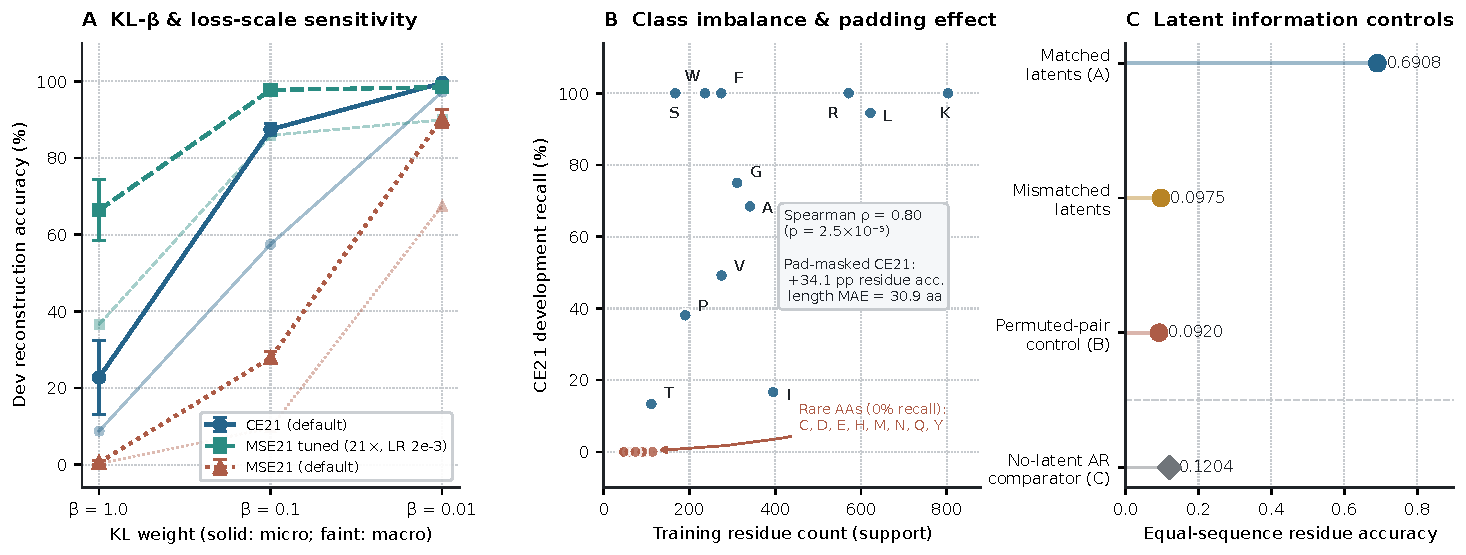
\includegraphics[width=\textwidth]{figures/fig2_kl_padding_and_latent_controls.pdf}
\caption{\rev{Diagnostic analyses of reconstruction sensitivity, class imbalance, padding and latent information. \textbf{(A)} Pilot KL-$\beta$ and MSE loss-scaling sweep (3 seeds, mean $\pm$ SD; solid lines: micro accuracy; faint lines: AA macro recall). Tuning MSE21 (21$\times$ loss scale, LR $2\times 10^{-3}$) bridges most of the micro gap, while CE21 retains a macro-recall advantage at $\beta=0.01$ ($p=0.0135$). \textbf{(B)} Per-amino-acid training support versus v7 1,000-step CE21 development recall (Spearman $\rho=0.80$, $p=2.5\times 10^{-5}$), with inset summarizing the 3-seed padding-masked ablation (+34.1 pp residue accuracy at the cost of length MAE 30.9 aa). \textbf{(C)} Latent-conditioned autoregression controls (equal-sequence residue accuracy): matched latents (0.6908) substantially exceed mismatched latents (0.0975), permuted-pair training (0.0920) and the capacity-unmatched no-latent comparator (0.1204), yet still failed generation-distance gates.}}\par\smallskip{\small\textbf{Alt text:} \rev{Three diagnostic panels. Panel A plots development reconstruction accuracy across beta 1.0, 0.1 and 0.01, showing CE21 and tuned MSE21 rising above 98 percent while default MSE21 lags. Panel B scatters training amino-acid counts against CE21 recall, showing rare residues at 0 percent and abundant residues near 100 percent (rho 0.80). Panel C shows four horizontal lollipops for latent-conditioned reconstruction controls, peaking at 0.6908 for matched latents versus 0.0920 to 0.1204 for controls.}}
\end{figure*}

\begin{figure*}[!t]
\centering
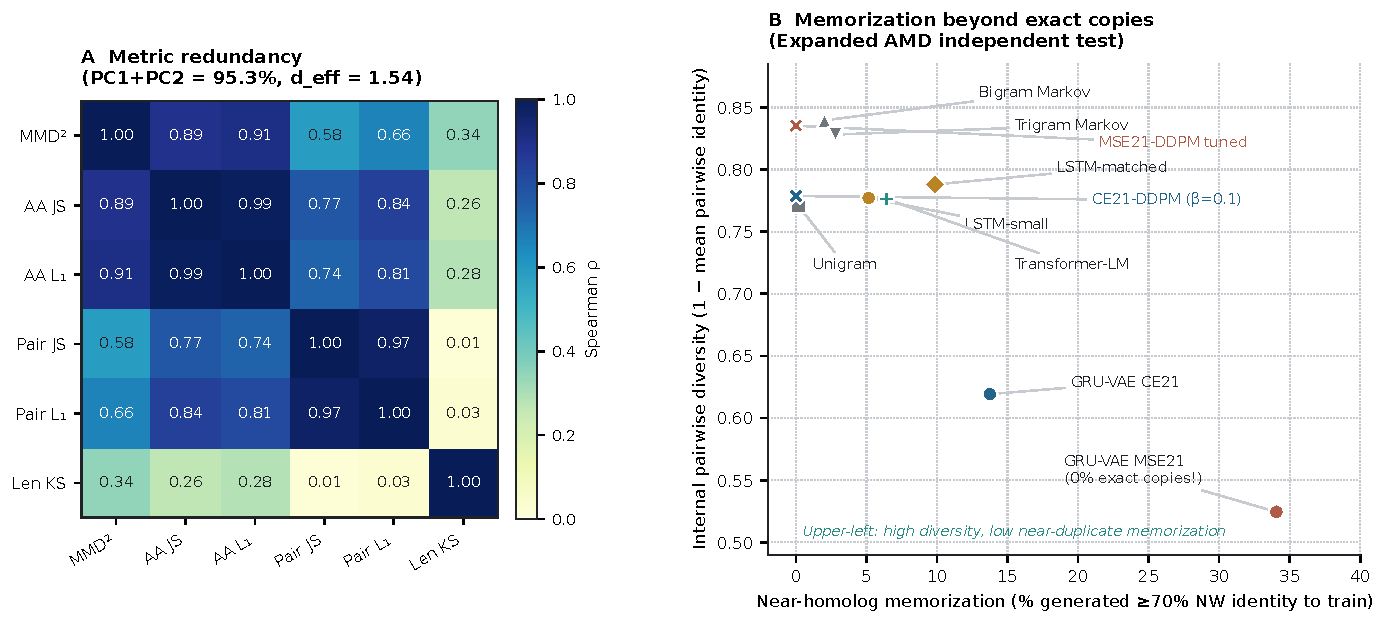
\includegraphics[width=\textwidth]{figures/fig3_memorization_diversity_and_corr.pdf}
\caption{\rev{Metric redundancy and near-duplicate memorization audits. \textbf{(A)} Spearman rank-correlation heatmap of the six low-order distributional distances across 160 model--seed--terminal runs (PC1+PC2 = 95.3\% variance; effective dimensionality $d_{\mathrm{eff}}=1.54$). \textbf{(B)} Near-homolog memorization (\% generated sequences with $\geq$70\% global Needleman--Wunsch identity to training) versus internal pairwise diversity on the expanded AMD independent test set. GRU-VAE MSE21 exhibits 34.1\% near-homolog collapse and reduced diversity (0.525) despite producing 0.0\% exact training copies.}}\par\smallskip{\small\textbf{Alt text:} \rev{Two-panel figure. Panel A is a 6-by-6 Spearman correlation heatmap showing strong correlations (0.74 to 0.99) among MMD squared, AA and dipeptide metrics, and weak correlation with length KS. Panel B scatters near-homolog memorization percentage against internal diversity, placing GRU-VAE MSE21 at the lower right (34.1 percent near-homologs, 0.525 diversity) and autoregressive and Markov models at the upper left.}}
\end{figure*}

\subsection{Exploratory latent diagnostics and activity-regression context}

\rev{To examine \emph{why} high reconstruction accuracy fails to translate into generation quality (Endpoint 1$\rightarrow$2) and whether in-silico predictors can replace laboratory assays (Endpoint 2$\rightarrow$3), we retained two exploratory diagnostic suites (Tables S3--S4). First, in latent-conditioned autoregression (\textbf{Figure 2C}), matched posterior latents achieved an eight-draw residue score of 0.6908 versus 0.0975 after latent mismatch and 0.0920 under permuted latent--sequence training (descriptive no-latent comparator: 0.1204), proving that the encoder preserves recoverable sequence information even though sampling failed generation criteria. Likewise, training-posterior substitution, coordinate permutation, KL warmup (0.7228$\rightarrow$0.6579), direct-latent diffusion and conditioning-context variants all failed pre-specified generation criteria (Table S4), pointing to latent-prior mismatch and non-autoregressive decoding rather than absent encoder information. Second, in source-group-held-out activity regression (Table S3), a QMAP-adapted CNN \cite{ref13,ref12} failed to outperform a training-weighted mean baseline on $\log_{10}$ MIC MAE in either mass units (0.8198 vs 0.8110; ridge 0.7754) or molar units (0.5763 vs 0.5170), and Gaussian right-censoring likelihood underperformed endpoint encoding across all weighting schemes. Although limited by small source-grouped caches ($n=46$--79), these diagnostics reinforce why quantitative in-silico MIC predictions cannot substitute for direct Endpoint-3 experimental assays.}

\subsection{Antibacterial activity and multi-threshold OD$_{600}$ audit in the 27-peptide panel}

In the separate 27-peptide experimental panel (all 27 tested under the confirmed MHB broth microdilution protocol; complete provenance in Table S5a), six peptides (22.2\%: pp1-3, pp1-5, pp2-8, pp3-11, pp3-13 and pp3-14) inhibited \textit{S. aureus} ATCC 29213 at MICs $\leq$31.25 \textmu{}g/mL, \rev{corresponding to potent molar MICs of 3.09--12.87 \textmu{}M (\textbf{Table 4}).} Two peptides, pp1-5 (7.8125 \textmu{}g/mL; 4.08 \textmu{}M) and pp3-13 (7.8125 \textmu{}g/mL; 3.09 \textmu{}M), showed the highest \textit{S. aureus} potency; pp1-5 also inhibited \textit{E. coli} (31.25 \textmu{}g/mL; 16.3 \textmu{}M), \textit{P. aeruginosa} (125 \textmu{}g/mL) and \textit{E. faecalis} (125 \textmu{}g/mL). Across all four strains, seven peptides (25.9\%) had MICs $<$200 \textmu{}g/mL against at least one strain. \rev{Consistent with cationic membrane-active AMP mechanisms, the six active hits carried substantially higher positive net charge at pH 7.4 than the 21 inactive peptides (mean $+4.30$ vs $+2.42$), while remaining sequence-novel (nearest-neighbor identity 36.0--44.4\% against pilot DBAASP). By design group, Group 1 (broad-spectrum, $n=7$) yielded 2 hits $\leq$31.25 \textmu{}g/mL (3 at $<$200 \textmu{}g/mL), Group 2 (Gram-positive, $n=8$) yielded 1 hit (pp2-8, Gram-positive selective), and Group 3 (intended Gram-negative-specific, $n=12$) yielded 3 hits active against both \textit{S. aureus} and \textit{E. coli} (0 strictly Gram-negative-only hits), illustrating that intended target-spectrum labels require experimental verification.}

\rev{Multi-threshold OD$_{600}$ sensitivity analysis across all 3,240 readings quantitatively justified the retrospective OD$_{600}<0.10$ cutoff (\textbf{Table 4}, \textbf{Figure 4}). Sterile blank medians spanned 0.0404--0.0435 across all four strains, whereas negative growth-control medians varied substantially by organism: 0.4942 (\textit{P. aeruginosa}), 0.2663 (\textit{E. coli}), 0.2230 (\textit{S. aureus}) and 0.1297 (\textit{E. faecalis}, minimum 0.1084). Consequently, OD$_{600}<0.10$ sits strictly below the minimum growth control of every strain and achieved peak concordance with the original reported summary (105/108 cells, 97.2\%; 3 discordant cells detailed in Table S5c). Crucially, the primary \textit{S. aureus} active count of \textbf{6/27 at $\leq$31.25 \textmu{}g/mL remained 100\% invariant across five distinct rules} (OD$_{600}<0.08, <0.10, <0.12$, and blank-normalized growth $<10\%$ and $<20\%$). Conversely, relaxing the fixed cutoff to OD$_{600}<0.15$ degraded concordance to 66/108 and inflated any-strain hits to 27/27 because \textit{E. faecalis} untreated growth controls frequently fell below 0.15---demonstrating why strain-specific control baselines are indispensable when auditing turbidimetric MIC data.}

\begin{table*}[t]
\caption{\rev{Endpoint-3 experimental audit: (Top) Multi-threshold OD$_{600}$ and blank-normalized growth sensitivity across all 3,240 readings (108 peptide--strain cells); (Bottom) Physicochemical, sequence-novelty and molar-MIC profile of the six \textit{S. aureus}-active peptides ($\leq$31.25 \textmu{}g/mL).}}
\label{tab:wetlab_summary}
\centering
\footnotesize
\begin{tabular}{lrrrrr}
\toprule
\multicolumn{6}{l}{\textit{\rev{A. Multi-threshold OD$_{600}$ sensitivity analysis (all denominators = 27 assayed peptides)}}} \\
\rev{Retrospective Endpoint Rule ($\geq$2/3 replicate consensus)} & \rev{Concordance (/108)} & \rev{\textit{S. aureus} $\leq$31.25} & \rev{\textit{S. aureus} $<$200} & \rev{Any $\leq$31.25} & \rev{Any $<$200} \\
\midrule
Original reported MIC summary & 108/108 (ref.) & 6/27 & 6/27 & 6/27 & 7/27 \\
\rev{Fixed OD$_{600}<0.08$} & \rev{99/108 (91.7\%)} & \rev{6/27} & \rev{6/27} & \rev{6/27} & \rev{6/27} \\
\rev{Fixed OD$_{600}<0.10$ (primary retrospective rule)} & \rev{\textbf{105/108 (97.2\%)}} & \rev{\textbf{6/27}} & \rev{7/27} & \rev{\textbf{6/27}} & \rev{\textbf{7/27}} \\
\rev{Fixed OD$_{600}<0.12$} & \rev{93/108 (86.1\%)} & \rev{6/27} & \rev{7/27} & \rev{7/27} & \rev{10/27} \\
\rev{Fixed OD$_{600}<0.15$ (fails on \textit{E. faecalis} ctrl 0.130)} & \rev{66/108 (61.1\%)} & \rev{9/27} & \rev{13/27} & \rev{27/27} & \rev{27/27} \\
\rev{Blank-normalized growth $<10\%$} & \rev{95/108 (88.0\%)} & \rev{6/27} & \rev{6/27} & \rev{6/27} & \rev{6/27} \\
\rev{Blank-normalized growth $<20\%$} & \rev{98/108 (90.7\%)} & \rev{6/27} & \rev{6/27} & \rev{6/27} & \rev{6/27} \\
\midrule
\multicolumn{6}{l}{\textit{\rev{B. Six \textit{S. aureus}-active hits ($\leq$31.25 \textmu{}g/mL; 0/27 overlap with AMPGen; haemolysis/cytotoxicity unmeasured)}}} \\
\rev{Peptide ID (Group) \& Sequence} & \rev{Purity (\%)} & \rev{Charge (pH 7.4)} & \rev{$\mu_H$ ($\alpha$-helix)} & \rev{NN id (DBAASP)} & \rev{\textit{S. aureus} MIC (\textmu{}g/mL / \textmu{}M)} \\
\midrule
\rev{pp1-3 (G1) \texttt{CVVSLFKSKKGGLRKHGVPFKL}} & \rev{95.6} & \rev{+5.74} & \rev{0.251} & \rev{40.9\%} & \rev{31.25 / 12.87 \textmu{}M} \\
\rev{pp1-5 (G1) \texttt{LKFTFIKGKFGKSSYY}} & \rev{96.1} & \rev{+3.79} & \rev{0.112} & \rev{37.5\%} & \rev{7.8125 / 4.08 \textmu{}M} \\
\rev{pp2-8 (G2) \texttt{FMPVVLTKLFGVLHFRKIY}} & \rev{97.8} & \rev{+2.84} & \rev{0.082} & \rev{42.1\%} & \rev{15.625 / 6.77 \textmu{}M} \\
\rev{pp3-11 (G3) \texttt{FKGVAKARHRLWFL}} & \rev{95.1} & \rev{+3.84} & \rev{0.314} & \rev{44.4\%} & \rev{15.625 / 9.04 \textmu{}M} \\
\rev{pp3-13 (G3) \texttt{KTFKKKLFLKLFYILHTPTY}} & \rev{95.4} & \rev{+4.84} & \rev{0.180} & \rev{41.4\%} & \rev{7.8125 / 3.09 \textmu{}M} \\
\rev{pp3-14 (G3) \texttt{CFANFQSKLHREARKLMGGAKKWPY}} & \rev{95.9} & \rev{+4.74} & \rev{0.496} & \rev{36.0\%} & \rev{31.25 / 10.53 \textmu{}M} \\
\bottomrule
\end{tabular}
\end{table*}

\begin{figure*}[!t]
\centering
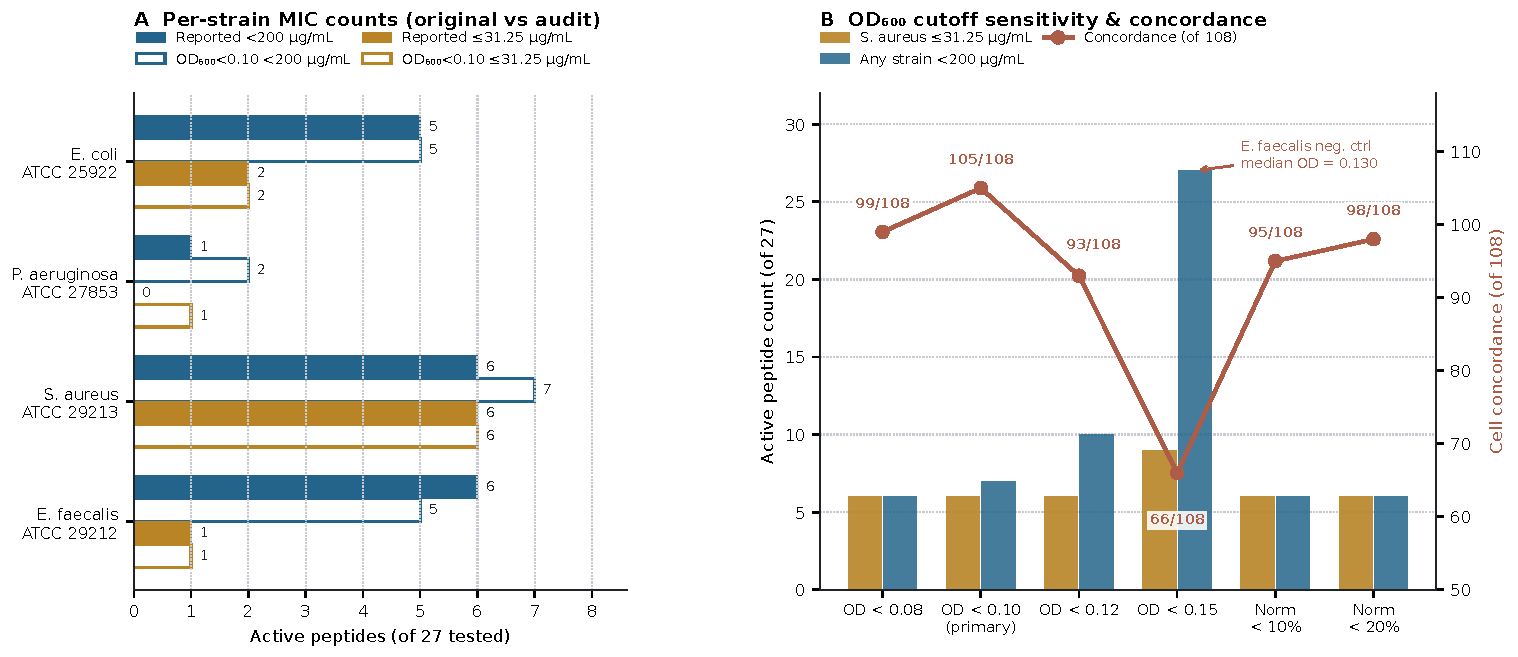
\includegraphics[width=\textwidth]{figures/fig4_mic_sensitivity_and_provenance.pdf}
\caption{\rev{Antibacterial activity of 27 tested peptides under the confirmed MHB broth microdilution protocol and multi-threshold OD$_{600}$ sensitivity audit. \textbf{(A)} Per-strain active peptide counts at $<$200 and $\leq$31.25 \textmu{}g/mL comparing the original reported MIC summary (filled) with the primary retrospective OD$_{600}<0.10$ consensus audit (outlined). \textbf{(B)} Six-rule sensitivity audit showing active counts (bars, left axis) and concordance with the 108 original cells (red line, right axis). The 6/27 \textit{S. aureus} $\leq$31.25 \textmu{}g/mL count is invariant across OD$_{600}<0.08, 0.10, 0.12$ and blank-normalized growth $<10\%$ and $<20\%$, whereas OD$_{600}<0.15$ fails on \textit{E. faecalis} (median negative-control OD$_{600}=0.130$). Complete peptide-level values are in Table S5.}}\par\smallskip{\small\textbf{Alt text:} \rev{Two-panel figure. Panel A shows horizontal paired bars of active peptides per strain for reported versus OD600 under 0.10 endpoints. Panel B combines vertical bars and a concordance line across six OD600 and normalized-growth thresholds, peaking at 105 of 108 concordance at OD600 under 0.10 and dropping to 66 of 108 at OD600 under 0.15 due to low Enterococcus faecalis control density.}}
\end{figure*}

\begin{figure*}[!t]
\centering
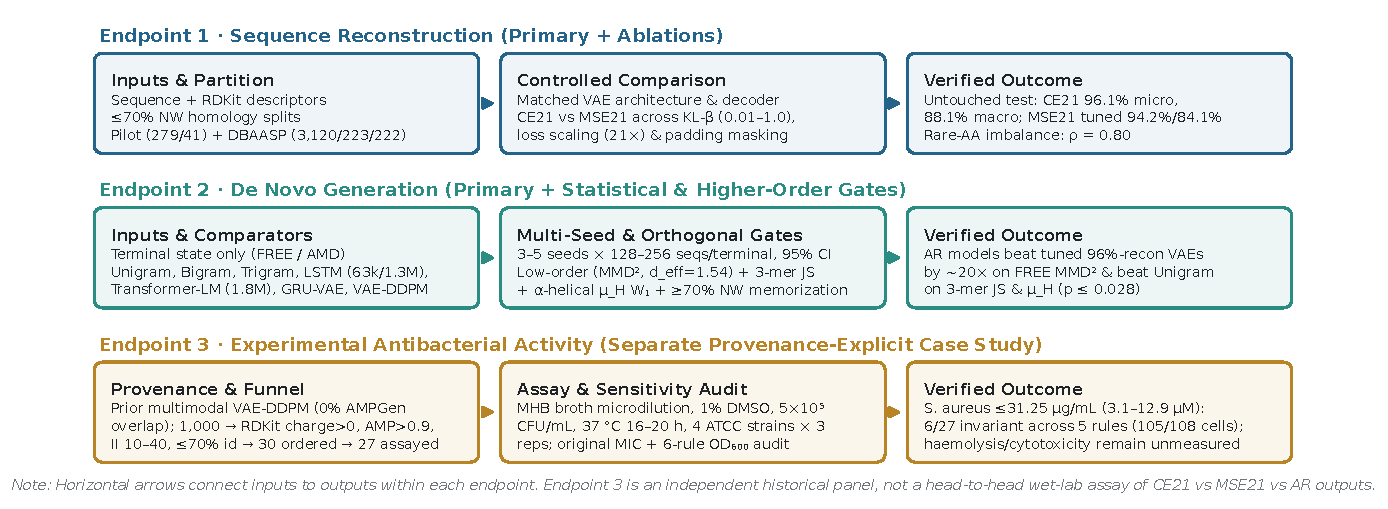
\includegraphics[width=\textwidth]{figures/fig5_endpoint_protocol.pdf}
\caption{\rev{Consolidated endpoint-specific evaluation protocol for antimicrobial peptide design. Three parallel tracks map inputs, controlled interventions and verified outcomes across Endpoint 1 (sequence reconstruction on homology-isolated splits), Endpoint 2 (multi-seed de novo generation with statistical baselines, capacity-matched autoregressive comparators and orthogonal fidelity/memorization gates) and Endpoint 3 (provenance-explicit broth microdilution assays with multi-threshold OD$_{600}$ sensitivity auditing and explicit safety-endpoint boundaries).}}\par\smallskip{\small\textbf{Alt text:} \rev{Three-row protocol diagram linking inputs, controlled comparisons and verified outcomes for sequence reconstruction, de novo generation and experimental antibacterial activity, with an explicit note that Endpoint 3 is an independent historical panel rather than a head-to-head assay of Endpoint 1 models.}}
\end{figure*}

\section{Discussion}

\rev{\subsection{Why separating reconstruction, sampling and activity matters in practice}}

\rev{Our expanded multi-seed benchmark on an untouched, homology-isolated test set transforms our initial descriptive observation into a robust methodological conclusion (\textbf{Figure 5}). First, comparing CE21 and MSE21 solely at a fixed default $\beta=1.0$ and unscaled loss $\alpha=0.5$ confounds objective choice with effective KL regularization: rescaling MSE21 by 21-fold with tuned learning rate and $\beta=0.1$ elevated its independent-test reconstruction accuracy from 5.24\% to 94.24\%, closely approaching CE21's 96.05\%. Even after tuning, however, CE21 retained higher macro recall across rare amino acids, and \emph{neither} 94\% nor 96\% reconstruction accuracy prevented latent-diffusion sampling from trailing capacity-matched LSTM-matched and Transformer-LM generators by roughly 20-fold on FREE MMD$^2$. This decoupling mirrors latent-variable-versus-sampling dissociations in discrete sequence VAEs \cite{refBowman}, reinforced by our latent-conditioned autoregression and padding-mask diagnostics: high encoder-decoder capacity on fixed padded grids does not guarantee a well-matched generative prior or natural length termination.}

\rev{Second, our expanded comparators reveal why multi-tier generation gates are indispensable. Had we evaluated only low-order MMD$^2$ without simple statistical baselines, we would have missed that zero-parameter Unigram sampling matches neural models on low-order composition ($0.00230$ vs $0.00323\text{--}0.00357$); conversely, adding tripeptide divergence and $\alpha$-helical hydrophobic moment ($\mu_H$) cleanly separated neural autoregressive models from Unigram ($p\leq 0.028$), while nearest-neighbor global alignment exposed severe hidden near-homolog collapse in GRU-VAE MSE21 (34.1\% $\geq$70\% identity despite 0.0\% exact copies). Together with our metric-redundancy audit ($d_{\mathrm{eff}}=1.54$ across the six low-order distances), these results show that AMP benchmarks should pair one primary low-order distance with orthogonal higher-order, amphipathic and alignment-based memorization metrics rather than multiplying correlated summary scores \cite{ref4,ref5,ref43,ref45}.}

\rev{\subsection{Interpreting the 27-peptide wet-lab panel and scope boundaries}}

\rev{Clarifying both the 1,000$\rightarrow$30$\rightarrow$27 screening funnel and the confirmed MHB broth microdilution protocol resolves experimental reproducibility while sharpening scientific attribution. Because the 27 candidates originated from an earlier multimodal VAE--diffusion model and passed stringent downstream filtering (net charge, AMP Scanner $>0.9$, instability index 10--40 and $\leq$70\% training similarity), their 22.2\% potent hit rate against \textit{S. aureus} ($\leq$31.25 \textmu{}g/mL; 3.09--12.87 \textmu{}M) reflects the \emph{combined} historical generation-plus-selection pipeline rather than a head-to-head wet-lab comparison of CE21, MSE21 and autoregressive outputs. In this respect, the panel serves the same endpoint-clarifying role as our comparison with AMPGen \cite{ref9}: it demonstrates Endpoint-3 reporting rigor (complete protocol parameters, tested-panel denominators, molar conversions and 6-rule OD$_{600}$ control auditing) without overclaiming model-level biological superiority.}

\rev{Important limitations bound these claims and define priorities for prospective work. First, our antibacterial panel measures in vitro planktonic growth inhibition only: \textbf{haemolytic activity (HC$_{50}$), mammalian cytotoxicity (CC$_{50}$), therapeutic selectivity indices, serum stability and in vivo efficacy were not measured} \cite{ref24,ref67,ref70}. Because strongly cationic, hydrophobic AMPs frequently exhibit host-membrane toxicity, the six active hits reported here must be regarded strictly as preliminary antibacterial leads requiring dedicated haemolysis and cytotoxicity profiling before any therapeutic interpretation. Second, although our computational benchmark now spans 3,565 homology-isolated DBAASP peptides across ten model configurations, direct head-to-head experimental validation linking fixed multi-seed generative outputs (without asymmetric post-hoc filtering) to paired MIC and haemolysis assays remains a prospective next step. Preserving explicit sequence, terminal-chemistry and assay metadata across public repositories such as DBAASP \cite{ref10}, APD3 \cite{ref60}, CAMPR4 \cite{ref63} and DRAMP 4.0 \cite{ref61} will make such end-to-end protocols directly comparable.}

\section{Conclusion}

\rev{Across both our original pilot cohort and an 11-fold larger, homology-isolated DBAASP independent test benchmark, multi-seed evaluation confirms that sequence reconstruction, de novo generation and antibacterial activity answer fundamentally distinct scientific questions. Proper KL-$\beta$ and loss-scale tuning elevates both CE21 and MSE21 to 94--96\% independent-test reconstruction while preserving a macro-recall edge for CE21, yet de novo generation remains dominated by capacity-matched autoregressive models (LSTM-matched, Transformer-LM and LSTM-small), which also significantly surpass statistical unigram sampling on tripeptide structure and $\alpha$-helical amphipathicity without hidden near-homolog collapse. Paired with a confirmed MHB broth microdilution protocol and six-rule OD$_{600}$ sensitivity audit on 27 sequence-novel candidates (six inhibiting \textit{S. aureus} at 3.09--12.87 \textmu{}M, with haemolysis and cytotoxicity unmeasured), this five-step protocol provides a rigorous, reproducible template for antimicrobial peptide design.}

\FloatBarrier
\section*{Author contributions}

\textbf{Hongsheng Wang:} Conceptualization, Methodology, Software, Validation, Formal analysis, Investigation, Data Curation, Writing -- Original Draft, Visualization.

\textbf{Zihan Zeng:} Z.H.Z. led wetlab experiments.

\textbf{Fei Wu:} Conceptualization (academic supervision), Writing -- Review \& Editing, Supervision, Project administration, Funding acquisition.

\textbf{Feng Lin:} Resources; Conceptualization (industrial scenario and requirements); Writing -- Review \& Editing; Supervision (industrial supervisor).

F.L. and X.X.H. conceived of the study and supervised its performance.

Fei Wu is the guarantor of the work.

\section*{Competing interests}

Hongsheng Wang's affiliation with Loctek Ergonomic Technology Corp. and the institutional collaborations are disclosed in the author list. The authors report no competing interests beyond these disclosed collaborations.

\section*{Relationship to prior work}
Hongsheng Wang, Zihan Zeng, Feng Lin and Xingxu Huang are also authors of AMPGen \cite{ref9}. \rev{As detailed in Table 1, the present study uses distinct generative architectures, separate computational datasets (including a newly frozen 3,565-peptide DBAASP benchmark), zero overlapping candidate peptide sequences (0/27) and separate antibacterial assay measurements, while sharing the same laboratory broth microdilution protocol.} AMPGen is cited as methodological context for staged candidate generation and biological assessment.

\section*{Ethics statement}

No human participants, human tissue or animal subjects were involved in this work. All bacterial work used the standard reference strains described in Materials and methods.

\section*{Data and code availability}
The versioned data and code for the initial submission are archived at Zenodo (\url{https://doi.org/10.5281/zenodo.23610740}) \cite{refData}, \rev{with the updated revision release (including the frozen 3,565-peptide homology-partitioned DBAASP snapshot, all multi-seed training/ablation scripts, statistical summary tables and deterministic figure-rendering code) maintained in the versioned GitHub repository (\url{https://github.com/wanghongsheng01/bib-amp-review-materials-20261023}) and archived upon revision acceptance.} Offline verification scripts reproduce all reported computational and assay summaries.

\section*{Acknowledgements and use of generative AI tools}

The authors wrote the manuscript. OpenAI Codex, Claude and \rev{Google Antigravity (Gemini)} assisted with source and reference checking, code inspection, independent recalculation of saved outputs, multi-seed experiment scripting, deterministic plotting code, factual verification and language editing of the author-written text. No fabricated laboratory measurements or generative images were created. Human authors verified all scientific claims against primary experimental records and retain full responsibility for the content.

\section*{Funding}

This work was supported by Zhejiang University. No other funding supported this work.

\section*{Supplementary material}
Supplementary Methods and Tables S1--\rev{S10} provide network architectures, molecular descriptor definitions, \rev{expanded DBAASP split hashes, multi-seed KL-$\beta$/padding ablations, full independent-test generation statistics with 95\% CIs, metric-correlation matrices, v7 large-sample replays,} activity-regression analyses, latent analyses, complete peptide-level MIC/OD$_{600}$ records and AMPGen context.

\noindent\begin{minipage}{\columnwidth}
\section*{Key Points}
\begin{itemize}
\item \rev{On a homology-isolated 3,565-peptide DBAASP benchmark (222 untouched test peptides, $<$70\% identity), KL-$\beta$ and 21-fold MSE scaling raise reconstruction to 96.1\% (CE21) and 94.2\% (MSE21 tuned), yet both VAE--diffusion models still trail capacity-matched autoregressive generators by $\sim$20-fold on FREE MMD$^2$.}
\item \rev{Six low-order distributional distances span only 1.54 effective dimensions (PC1+PC2 = 95.3\%); tripeptide divergence, $\alpha$-helical hydrophobic moment ($\mu_H$) and $\geq$70\% nearest-neighbor alignment identity are required to separate neural models from unigram baselines ($p\leq 0.028$) and expose hidden near-duplicate memorization (up to 34.1\% at 0\% exact copies).}
\item \rev{Under a confirmed Mueller--Hinton broth microdilution protocol (1\% DMSO, $5\times 10^5$ CFU/mL, 37~$^\circ$C, 16--20 h), 6/27 sequence-novel peptides inhibit \textit{S. aureus} at $\leq$31.25 \textmu{}g/mL (3.09--12.87 \textmu{}M), invariant across five OD$_{600}$ and normalized-growth thresholds; haemolysis and cytotoxicity remain unmeasured.}
\item \rev{A consolidated five-step protocol separates Primary, Exploratory and Retrospective evidence across reconstruction, generation and antibacterial endpoints.}
\end{itemize}
\end{minipage}

\begin{thebibliography}{99}
\bibitem{ref50} Magana M, Pushpanathan M, Santos AL, et al. The value of antimicrobial peptides in the age of resistance. \textit{Lancet Infect Dis} 2020;20:e216--30. doi:10.1016/S1473-3099(20)30327-3. PMID: 32653070.
\bibitem{ref51} Lazzaro BP, Zasloff M, Rolff J. Antimicrobial peptides: application informed by evolution. \textit{Science} 2020;368:eaau5480. doi:10.1126/science.aau5480. PMID: 32355003. PMCID: PMC8097767.
\bibitem{ref1} Müller AT, Hiss JA, Schneider G. Recurrent neural network model for constructive peptide design. \textit{J Chem Inf Model} 2018;58:472--9. doi:10.1021/acs.jcim.7b00414. PMID: 29355319.
\bibitem{ref16} Dean SN, Walper SA. Variational autoencoder for generation of antimicrobial peptides. \textit{ACS Omega} 2020;5:20746--54. doi:10.1021/acsomega.0c00442. PMID: 32875208. PMCID: PMC7450509.
\bibitem{ref17} Dean SN, Alvarez JAE, Zabetakis D, et al. PepVAE: variational autoencoder framework for antimicrobial peptide generation and activity prediction. \textit{Front Microbiol} 2021;12:725727. doi:10.3389/fmicb.2021.725727. PMID: 34659152. PMCID: PMC8515052.
\bibitem{ref2} Szymczak P, Możejko M, Grzegorzek T, et al. Discovering highly potent antimicrobial peptides with deep generative model HydrAMP. \textit{Nat Commun} 2023;14:1453. doi:10.1038/s41467-023-36994-z. PMID: 36922490. PMCID: PMC10017685.
\bibitem{ref15} Van Oort CM, Ferrell JB, Remington JM, et al. AMPGAN v2: machine learning-guided design of antimicrobial peptides. \textit{J Chem Inf Model} 2021;61:2198--207. doi:10.1021/acs.jcim.0c01441. PMID: 33787250. PMCID: PMC8281497.
\bibitem{ref19} Yu H, Wang R, Qiao J, et al. Multi-CGAN: Deep Generative Model-Based Multiproperty Antimicrobial Peptide Design. \textit{J Chem Inf Model} 2024;64:316--326. doi:10.1021/acs.jcim.3c01881.
\bibitem{ref9} Jin S, Zeng Z, Xiong X, et al. AMPGen: an evolutionary information-reserved and diffusion-driven generative model for de novo design of antimicrobial peptides. \textit{Commun Biol} 2025;8:839. doi:10.1038/s42003-025-08282-7. PMID: 40447738. PMCID: PMC12125351.
\bibitem{ref11} Cao J, Zhang J, Yu Q, et al. TG-CDDPM: text-guided antimicrobial peptides generation based on conditional denoising diffusion probabilistic model. \textit{Brief Bioinform} 2025;26:bbae644. doi:10.1093/bib/bbae644. PMID: 39668337. PMCID: PMC11637771.
\bibitem{ref20} Wang XF, Tang JY, Sun J, et al. ProT-Diff: a modularized and efficient strategy for de novo generation of antimicrobial peptide sequences by integrating protein language and diffusion models. \textit{Adv Sci} 2024;11:e2406305. doi:10.1002/advs.202406305. PMID: 39319609. PMCID: PMC11578372.
\bibitem{ref21} Wang R, Wang T, Zhuo L, et al. Diff-AMP: tailored designed antimicrobial peptide framework with all-in-one generation, identification, prediction and optimization. \textit{Brief Bioinform} 2024;25:bbae078. doi:10.1093/bib/bbae078. PMID: 38446739. PMCID: PMC10939340.
\bibitem{refLe2022} \rev{Le NQK. Potential of deep representative learning features to interpret the sequence information in proteomics. \textit{Proteomics} 2022;22(1--2):e2100232. doi:10.1002/pmic.202100232. PMID: 34730875.}
\bibitem{refLe2021} \rev{Le NQK, Do DT, Nguyen TT, Le QA. A sequence-based prediction of Kruppel-like factors proteins using XGBoost and optimized features. \textit{Gene} 2021;787:145643. doi:10.1016/j.gene.2021.145643. PMID: 33848577.}
\bibitem{refAMPScanner} \rev{Veltri D, Kamath U, Shehu A. Deep learning improves antimicrobial peptide recognition. \textit{Bioinformatics} 2018;34:2740--2747. doi:10.1093/bioinformatics/bty179. PMID: 29590297. PMCID: PMC6084614.}
\bibitem{ref14} Das P, Sercu T, Wadhawan K, et al. Accelerated antimicrobial discovery via deep generative models and molecular dynamics simulations. \textit{Nat Biomed Eng} 2021;5:613--23. doi:10.1038/s41551-021-00689-x. PMID: 33707779.
\bibitem{refCao2023} Cao Q, Ge C, Wang X, et al. Designing antimicrobial peptides using deep learning and molecular dynamic simulations. \textit{Brief Bioinform} 2023;24:bbad058. doi:10.1093/bib/bbad058.
\bibitem{ref22} Huang J, Xu Y, Xue Y, et al. Identification of potent antimicrobial peptides via a machine-learning pipeline that mines the entire space of peptide sequences. \textit{Nat Biomed Eng} 2023;7:797--810. doi:10.1038/s41551-022-00991-2.
\bibitem{ref25} Sun Z, Wang X, Kuang S, et al. From generation to validation: Deep generative models for antimicrobial peptide discovery. \textit{Curr Opin Chem Biol} 2026;93:102685. doi:10.1016/j.cbpa.2026.102685.
\bibitem{ref26} Polykovskiy D, Zhebrak A, Sanchez-Lengeling B, et al. Molecular Sets (MOSES): a benchmarking platform for molecular generation models. \textit{Front Pharmacol} 2020;11:565644. doi:10.3389/fphar.2020.565644. PMID: 33390943. PMCID: PMC7775580.
\bibitem{ref28} Brown N, Fiscato M, Segler MHS, et al. GuacaMol: benchmarking models for de novo molecular design. \textit{J Chem Inf Model} 2019;59:1096--108. doi:10.1021/acs.jcim.8b00839. PMID: 30887799.
\bibitem{ref29} Møller-Larsen R, Izdebski A, Olszewski J, et al. seqme: a Python library for evaluating biological sequence design from generative models. \textit{Bioinform Adv} 2026;6:vbag212. doi:10.1093/bioadv/vbag212. PMID: 42633207. PMCID: PMC13499220.
\bibitem{ref8} Beierle L, Hahnfeld J, Goesmann A, et al. Generative models for antimicrobial peptide design: auto-encoders and beyond. \textit{BioData Min} 2026;19:42. doi:10.1186/s13040-026-00558-w.
\bibitem{refXu2021} Xu J, Li F, Leier A, et al. Comprehensive assessment of machine learning-based methods for predicting antimicrobial peptides. \textit{Brief Bioinform} 2021;22:bbab083. doi:10.1093/bib/bbab083.
\bibitem{ref4} García-Jacas CR, Pinacho-Castellanos SA, García-González LA, Brizuela CA. Do deep learning models make a difference in the identification of antimicrobial peptides? \textit{Brief Bioinform} 2022;23:bbac094. doi:10.1093/bib/bbac094. PMID: 35380616.
\bibitem{ref5} Sidorczuk K, Gagat P, Pietluch F, et al. Benchmarks in antimicrobial peptide prediction are biased due to the selection of negative data. \textit{Brief Bioinform} 2022;23:bbac343. doi:10.1093/bib/bbac343. PMID: 35988923. PMCID: PMC9487607.
\bibitem{ref39} Teufel F, Gíslason MH, Almagro Armenteros JJ, et al. GraphPart: homology partitioning for biological sequence analysis. \textit{NAR Genom Bioinform} 2023;5:lqad088. doi:10.1093/nargab/lqad088. PMID: 37850036. PMCID: PMC10578201.
\bibitem{ref40} Kapoor S, Narayanan A. Leakage and the reproducibility crisis in machine-learning-based science. \textit{Patterns} 2023;4:100804. doi:10.1016/j.patter.2023.100804. PMID: 37720327. PMCID: PMC10499856.
\bibitem{ref43} Walsh I, Fishman D, Garcia-Gasulla D, et al. DOME: recommendations for supervised machine learning validation in biology. \textit{Nat Methods} 2021;18:1122--7. doi:10.1038/s41592-021-01205-4. PMID: 34316068.
\bibitem{ref44} Heil BJ, Hoffman MM, Markowetz F, et al. Reproducibility standards for machine learning in the life sciences. \textit{Nat Methods} 2021;18:1132--5. doi:10.1038/s41592-021-01256-7. PMID: 34462593. PMCID: PMC9131851.
\bibitem{ref45} Weber LM, Saelens W, Cannoodt R, et al. Essential guidelines for computational method benchmarking. \textit{Genome Biol} 2019;20:125. doi:10.1186/s13059-019-1738-8. PMID: 31221194. PMCID: PMC6584985.
\bibitem{ref13} Lavertu A, Corbeil J, Germain P. QMAP: a benchmark for standardized evaluation of antimicrobial peptide MIC and hemolytic activity regression. \textit{Sci Rep} 2026;16:25387. doi:10.1038/s41598-026-56004-8.
\bibitem{refLLAMP} Bae D, Kim M, Seo J, Nam H. AI-guided discovery and optimization of antimicrobial peptides through species-aware language model. \textit{Brief Bioinform} 2025;26:bbaf343. doi:10.1093/bib/bbaf343. PMID: 40676915. PMCID: PMC12271573.
\bibitem{ref10} Pirtskhalava M, Amstrong AA, Grigolava M, et al. DBAASP v3: database of antimicrobial/cytotoxic activity and structure of peptides as a resource for development of new therapeutics. \textit{Nucleic Acids Res} 2021;49:D288--97. doi:10.1093/nar/gkaa991. PMID: 33151284. PMCID: PMC7778994.
\bibitem{refNW} Needleman SB, Wunsch CD. A general method applicable to the search for similarities in the amino acid sequence of two proteins. \textit{J Mol Biol} 1970;48:443--53. doi:10.1016/0022-2836(70)90057-4.
\bibitem{refVAE} Kingma DP, Welling M. Auto-Encoding Variational Bayes. \textit{arXiv} 2013;1312.6114. doi:10.48550/arXiv.1312.6114.
\bibitem{refDDPM} Ho J, Jain A, Abbeel P. Denoising Diffusion Probabilistic Models. \textit{Adv Neural Inf Process Syst} 2020;33:6840--51.
\bibitem{refLSTM} Hochreiter S, Schmidhuber J. Long short-term memory. \textit{Neural Comput} 1997;9:1735--80. doi:10.1162/neco.1997.9.8.1735.
\bibitem{refJS} Lin J. Divergence measures based on the Shannon entropy. \textit{IEEE Trans Inf Theory} 1991;37:145--51. doi:10.1109/18.61115.
\bibitem{refMMD} Gretton A, Borgwardt KM, Rasch MJ, et al. A kernel two-sample test. \textit{J Mach Learn Res} 2012;13:723--73.
\bibitem{refEisenberg} \rev{Eisenberg D, Weiss RM, Terwilliger TC. The helical hydrophobic moment: a measure of the amphiphilicity of a helix. \textit{Nature} 1982;299:371--374. doi:10.1038/299371a0. PMID: 7110359.}
\bibitem{refBoman} \rev{Boman HG. Antibacterial peptides: basic facts and emerging concepts. \textit{J Intern Med} 2003;254:197--215. doi:10.1046/j.1365-2796.2003.01228.x. PMID: 12930229.}
\bibitem{ref12} Witten J, Witten Z. Deep learning regression model for antimicrobial peptide design. \textit{bioRxiv} 2019;692681. doi:10.1101/692681. Preprint.
\bibitem{ref64} Wiegand I, Hilpert K, Hancock REW. Agar and broth dilution methods to determine the minimal inhibitory concentration (MIC) of antimicrobial substances. \textit{Nat Protoc} 2008;3:163--75. doi:10.1038/nprot.2007.521. PMID: 18274517.
\bibitem{ref65} Balouiri M, Sadiki M, Ibnsouda SK. Methods for in vitro evaluating antimicrobial activity: a review. \textit{J Pharm Anal} 2016;6:71--9. doi:10.1016/j.jpha.2015.11.005. PMID: 29403965. PMCID: PMC5762448.
\bibitem{ref66} Meurer M, O'Neil DA, Lovie E, et al. Antimicrobial susceptibility testing of antimicrobial peptides requires new and standardized testing structures. \textit{ACS Infect Dis} 2021;7:2205--8. doi:10.1021/acsinfecdis.1c00210. PMID: 34110786. PMCID: PMC8764967.
\bibitem{refBowman} Bowman SR, Vilnis L, Vinyals O, et al. Generating Sentences from a Continuous Space. In: \textit{Proceedings of the 20th SIGNLL Conference on Computational Natural Language Learning.} Berlin: Association for Computational Linguistics, 2016, 10--21. doi:10.18653/v1/K16-1002.
\bibitem{ref24} Capecchi A, Cai X, Personne H, et al. Machine learning designs non-hemolytic antimicrobial peptides. \textit{Chem Sci} 2021;12:9221--9232. doi:10.1039/d1sc01713f.
\bibitem{ref60} Wang G, Li X, Wang Z. APD3: the antimicrobial peptide database as a tool for research and education. \textit{Nucleic Acids Res} 2016;44:D1087--93. doi:10.1093/nar/gkv1278.
\bibitem{ref63} Gawde U, Chakraborty S, Waghu FH, et al. CAMPR4: a database of natural and synthetic antimicrobial peptides. \textit{Nucleic Acids Res} 2023;51:D377--D383. doi:10.1093/nar/gkac933.
\bibitem{ref61} Ma T, Liu Y, Yu B, et al. DRAMP 4.0: an open-access data repository dedicated to the clinical translation of antimicrobial peptides. \textit{Nucleic Acids Res} 2025;53:D403--D410. doi:10.1093/nar/gkae1046.
\bibitem{ref67} Haney EF, Straus SK, Hancock REW. Reassessing the host defense peptide landscape. \textit{Front Chem} 2019;7:43. doi:10.3389/fchem.2019.00043. PMID: 30778385. PMCID: PMC6369191.
\bibitem{ref70} Timmons PB, Hewage CM. HAPPENN is a novel tool for hemolytic activity prediction for therapeutic peptides which employs neural networks. \textit{Sci Rep} 2020;10:10869. doi:10.1038/s41598-020-67701-3. PMID: 32616760. PMCID: PMC7331684.
\bibitem{refData} Wang H, Zeng Z, Wu F, Lin F, Huang X. Data and code for Separating reconstruction, generation and antibacterial activity in antimicrobial peptide design [data set and software]. Version v7-2026-10-24. Zenodo, 24 October 2026. doi:10.5281/zenodo.23610740.
\end{thebibliography}

\end{document}
